%%%%%%%%%%%%%%%%%%%%%%%%%%%%%%%%%%%%%%%%%%%%%%%%%%%%%%%%%%%%%%%%
%  Build your own EEDURO Delta Robot                           %
%                                                              %
%  Stefan Landis (stefan.landis@ntb.ch)                        %
%  Martin Züger (martin.zueger@ntb.ch)                         %
%%%%%%%%%%%%%%%%%%%%%%%%%%%%%%%%%%%%%%%%%%%%%%%%%%%%%%%%%%%%%%%%

% 1. Definieren der Dokumentklasse.
\documentclass[
  pdftex,                           % PDFTex verwenden um ausschliesslich ein PDF zu erzeugen
  a4paper,                          % A4 Papier
  doubleside,                       % Doppelseitiger Druck
  11pt,                             % Standard Schriftgrösse
  parskip=half,                     % Europäischer Satz mit Abstand zwischen Absätzen
  headsepline,                      % Linie nach Kopfzeile
  ]{scrreprt}                       % KOMA-Script Klasse

% 2. Zeichencodierung und Zeichensatz
\usepackage[utf8]{inputenc}         % 'utf8' -> nicht kompatibel mit TeXnicCenter (unterstützt kein UTF-8)
\usepackage[T1]{fontenc}            % 'T1' Codierung für die Schrift

% 3. Lokalisierung
\usepackage[english, american]{babel}
\usepackage{textcomp}               % Euro Symbol (\texteuro}
\usepackage{upgreek}				% Paket für nichtkursive griechische Kleinbuchstaben

% 4. Schriften
\usepackage{courier}                % Courier laden (wird für Code verwendet)
\usepackage{helvet}                 % Helvetica laden

% 5. Textpakete und Optionen
\usepackage{setspace}               % Paket für Textabstände
\onehalfspacing                     % 1.5-facher Zeilenabstand
\usepackage[section]{placeins}      % Paket für Flusskontrolle -> verhindert, das Flussobjekte aus
                                    % einer Section heraus geschoben werden
\usepackage{enumerate}

% 6. Seiteneinstellungen
\topmargin-12mm                     % Oberer Seitenrand verstellen -> Hack, verbessern
\headheight0.95cm                   % Höhe der Kopfzeile
\textheight24.2cm                   % Texthöhe (ohne Kopf- und Fusszeile)
\footskip1.2cm                      % Abstand zwischen Text und unterem Ende der Fusszeile
\raggedbottom                       % Kein vertikaler Blocksatz

% 7. Kopf-/Fusszeilen, Fussnoten
\usepackage{scrpage2}
\usepackage{remreset}
\makeatletter
\@removefromreset{footnote}{chapter}
\makeatother

% 8. Bilder, Tabellen, Boxen
\usepackage[pdftex]{graphicx}       % Bilder
\usepackage{booktabs}               % mehrere Befehle für die Tabellen
\usepackage{array}
\usepackage{framed}                 % Paket für Boxen
\usepackage{pdfpages}
\graphicspath{                      % Suchpfade für Bilder
  {img/},
  {Bilder/},
  {Grafiken/},
  {images/},
  {template/},
  {Img/},
  {abb/},
  {}}
\usepackage[format=hang,justification=centering]{caption}   
\usepackage{csvsimple}

% 9. Farben
\usepackage{color}                  % Paket für Farben laden
\definecolor{LinkColor}{rgb}{0,0,0} % Verschiedene Farbdefinitionen
\definecolor{darkblue}{rgb}{0,0,0.6}
\definecolor{darkred}{rgb}{0.6,0,0}
\definecolor{darkgreen}{rgb}{0,0.6,0}
\definecolor{red}{rgb}{0.98,0,0}
\definecolor{lstbggray}{rgb}{0.95,0.95,0.95}
\definecolor{gray50}{rgb}{0.5,0.5,0.5}

\definecolor{ntblightgray}{gray}{0.8}
\definecolor{ntbdarkgray}{gray}{0.7}
\definecolor{ntbblue}{cmyk}{1, 0.45, 0, 0.18}
\definecolor{ntblightblue}{cmyk}{0.55, 0.28, 0.05, 0.0}

% 10. Mathematik
\usepackage{amsmath}                % Verbesserter Mathematik Satz
\usepackage{amssymb}                % Zahlenmenngen in der Mathematik
\usepackage{trfsigns}               % Zeichen für Transformationen
\usepackage{mathptmx}               % Times New Roman für Mathematik

% 11. Codesegmente
\usepackage{listings}
\lstdefinelanguage{kmake}{
  keywords={ifeq, else, endif},
  morekeywords={},
  otherkeywords={},
  sensitive=true,
  comment=[l]{\#},
  string=[s]{"}{"},
  showspaces=false,
}
\lstloadlanguages{C, kmake}          % benötigte Sprachen laden
\lstset{                            % Einstellungen für C
  language=C,
  basicstyle=\scriptsize\ttfamily,
  commentstyle=\color{darkgreen},
  keywordstyle=\bfseries\color{darkblue},
  stringstyle=\color{darkred},
%  showspaces=false,
  columns=fixed,
  numbers=left,
%  frame=none,
  numberstyle=\tiny,
  breaklines=true,
%  captionpos=b,
  showstringspaces=false,
% xleftmargin=1cm,
  tabsize=4,
  backgroundcolor=\color{lstbggray},
  numberbychapter=false
}

\let\verbatimorg\verbatim
\renewcommand\verbatim{\small\verbatimorg}


% 12. Metadaten
\title{EEDURO User Manual}
\author{Martin Züger, Stefan Landis}
\date{\today}

% 13. PDF-Einstellungen
\usepackage[
  pdftitle={Build your own EEDURO Delta},
  pdfauthor={Martin Zueger, Stefan Landis},
  pdfcreator={Kile (http://kile.sourceforge.net)},
  pdfsubject={User Manual},
  pdfkeywords={NTB, EEROS, EEDURO, Delta, Robot},
  pdfpagemode=UseOutlines,          % Inhaltsverzeichnis anzeigen beim öffnen
  pdfdisplaydoctitle=true           % Dokumenttitel statt Dateiname anzeigen
  ]{hyperref}
\hypersetup{
  colorlinks=true,
  linkcolor=LinkColor,              % Farbe für Links
  citecolor=LinkColor,              % Farbe für Literaturreferenzen
  filecolor=LinkColor,              % 
  menucolor=LinkColor,              % 
  pagecolor=LinkColor,              % Farbe für Links auf Seitenzahlen
  urlcolor=LinkColor}               % Farbe für URLs

% 14. Eigene Befehle
% 14.1. Text überstreichen
\newcommand{\OL}[1]{$\overline{\text{#1}}$}


\begin{document}

\begin{titlepage}
	\begin{center}
		
\includegraphics[height=2cm]{EEROS_Logo}
	\end{center}
	\vspace{4.5cm}
	{
		\fontfamily{phv}\selectfont
	
		\rule{\linewidth}{0.5mm} \\[0cm]
	
		\begin{center}
			{\huge \bfseries Build your own EEDURO Delta} \\
		\end{center}
		
		\rule{\linewidth}{0.5mm} \\[0.4cm]
		
		\vspace{1.5cm}
		
		Stefan Landis, Martin Züger \\
		
		
		NTB University of Applied Sciences of Technology Buchs\\
		Werdenbergstrasse 4\\
		9471 Buchs\\
		Switzerland\\
		\vfill
	}
\end{titlepage}
\clearpage

\begin{abstract}

\begin{large}
 \textbf{Document Revisions}
\end{large}

\begin{tabular}{|l|l|l|p{10cm}|}
\hline
\textbf{Rev.} & \textbf{Date} & \textbf{Author} & \textbf{Changes} \\
\hline
0.1 & 2015-02-04 & Martin Zueger & Initial version \\
\hline
\end{tabular} 
%\thispagestyle{empty}

\end{abstract}
\setcounter{page}{1}
\setcounter{tocdepth}{2}
\tableofcontents

\newpage

\chapter{Introduction}
TODO Stefan/Martin

\chapter{Getting all necessary parts}

\section{Manufactering the mechanical parts}
TODO Stefan

\section{Ordering the commercial parts}
TODO Stefan/Martin

\chapter{Mechanical assembly}

\section{EEDURO Delta robot}

\begin{figure}[htbp]
	\centering
	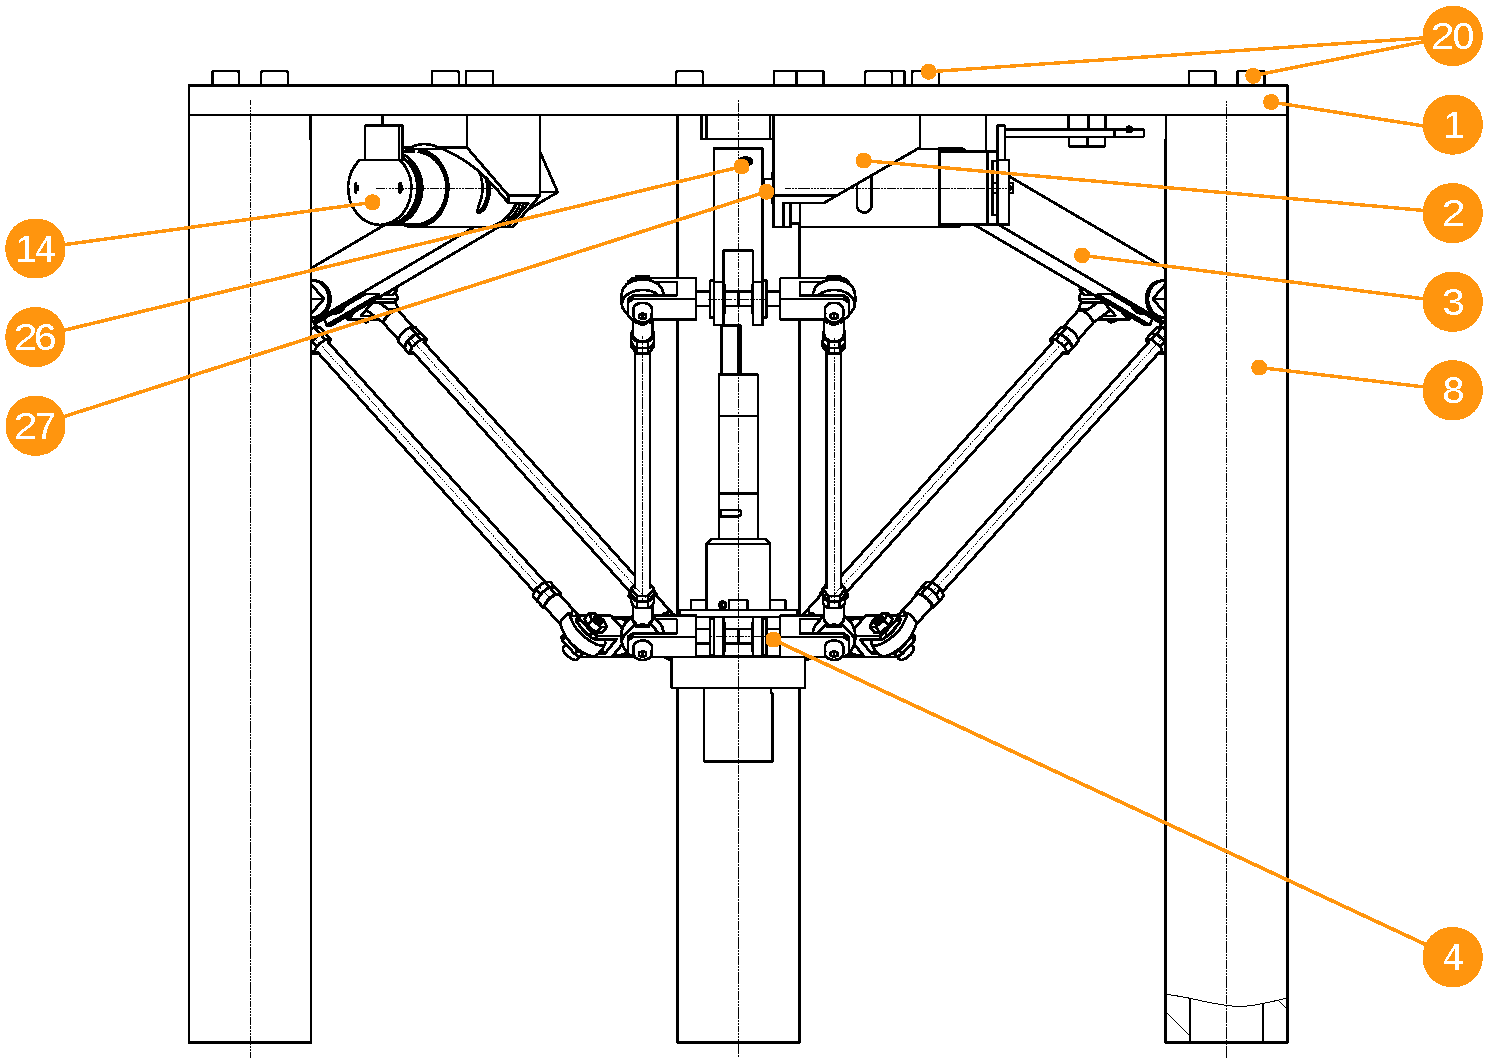
\includegraphics[width=\textwidth]{DeltaMechanicalPartsOverview}
	\caption{EEDURO delta}
	\label{fig:DeltaMechanicalPartsOverview}
\end{figure}

\begin{figure}[htbp]
	\centering
	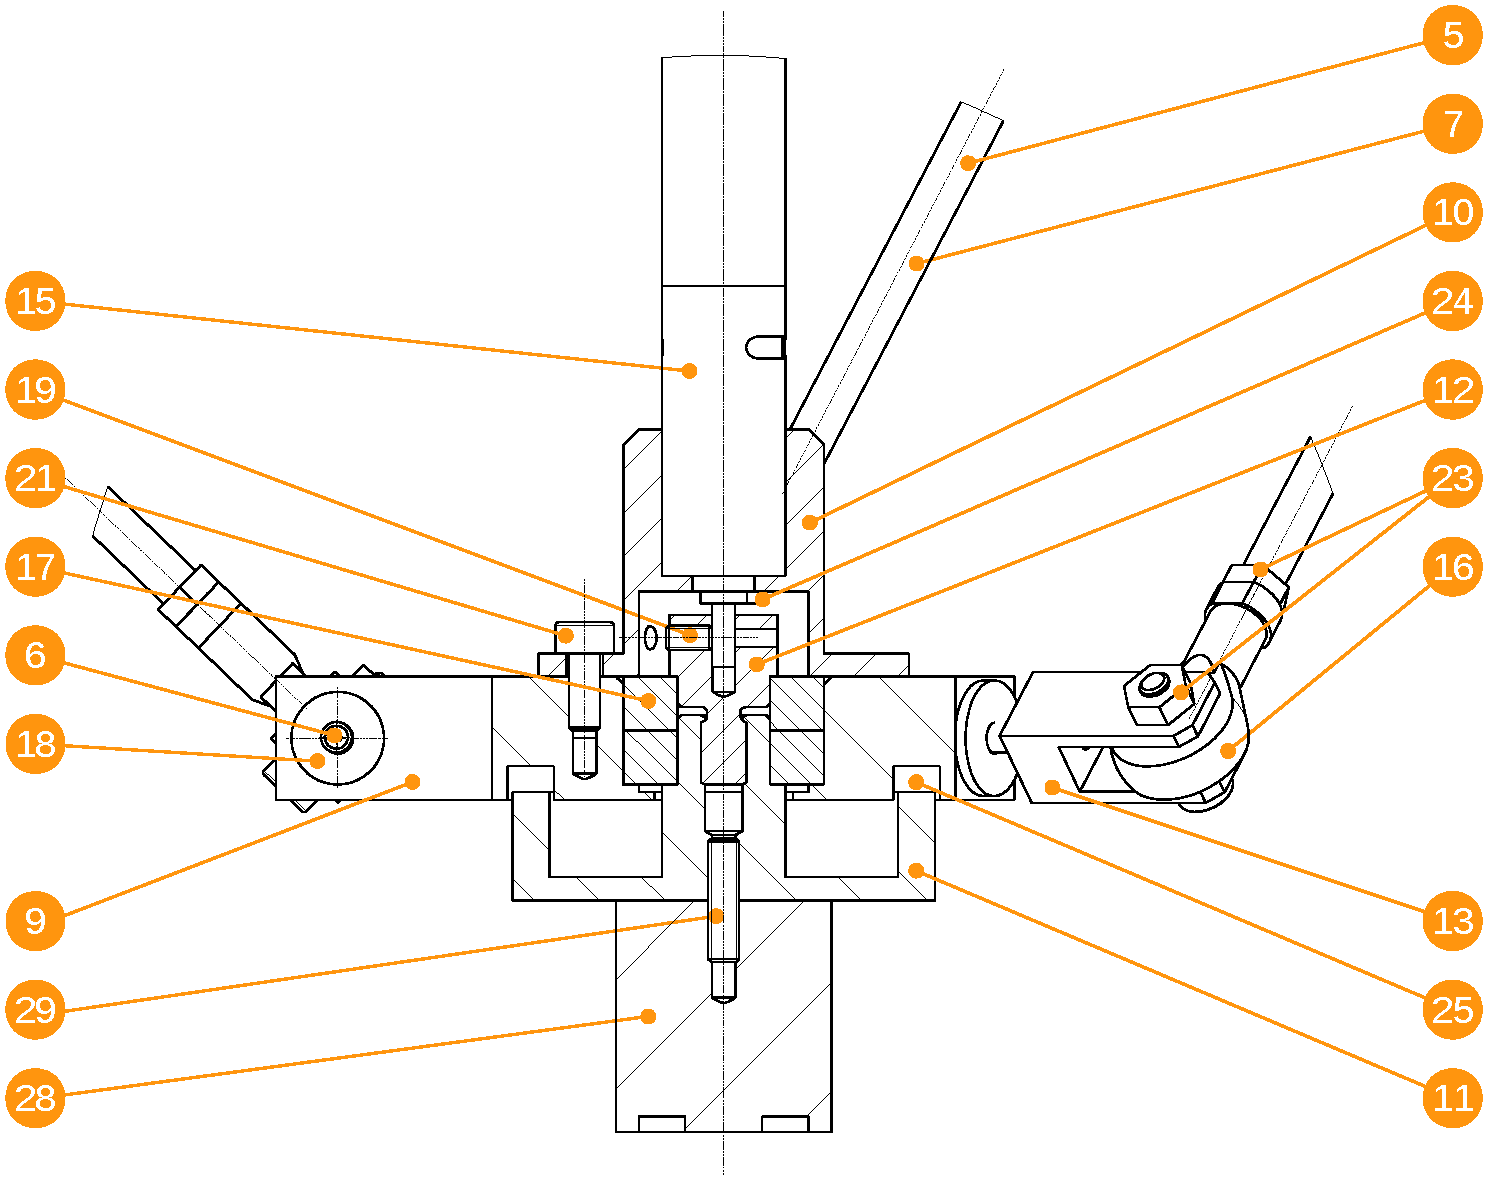
\includegraphics[width=\textwidth]{DeltaMechanicalPartsOverviewTCP}
	\caption{EEDURO delta TCP detail view (with mounted electro magnet)}
	\label{fig:DeltaMechanicalPartsOverviewTCP}
\end{figure}

\subsection*{Step 1: Mount the electro magnet}

\begin{minipage}[t]{0.6\textwidth}
	\begin{itemize}
		\item Remove the heat shrink tubing from the cable of the electromagnets.
		\item Screw the rotating tool carrier (11) and the electromagnet (28) with the grub screw M2x8 (29) together and fix them with Loctite. 
		\item Wind the cable of the electromagnet at least three or four times around the thicker flange of the tool carrier.
	\end{itemize}
\end{minipage}
\hfill
\begin{minipage}[t]{0.35\textwidth}
	\vspace{-\ht\strutbox}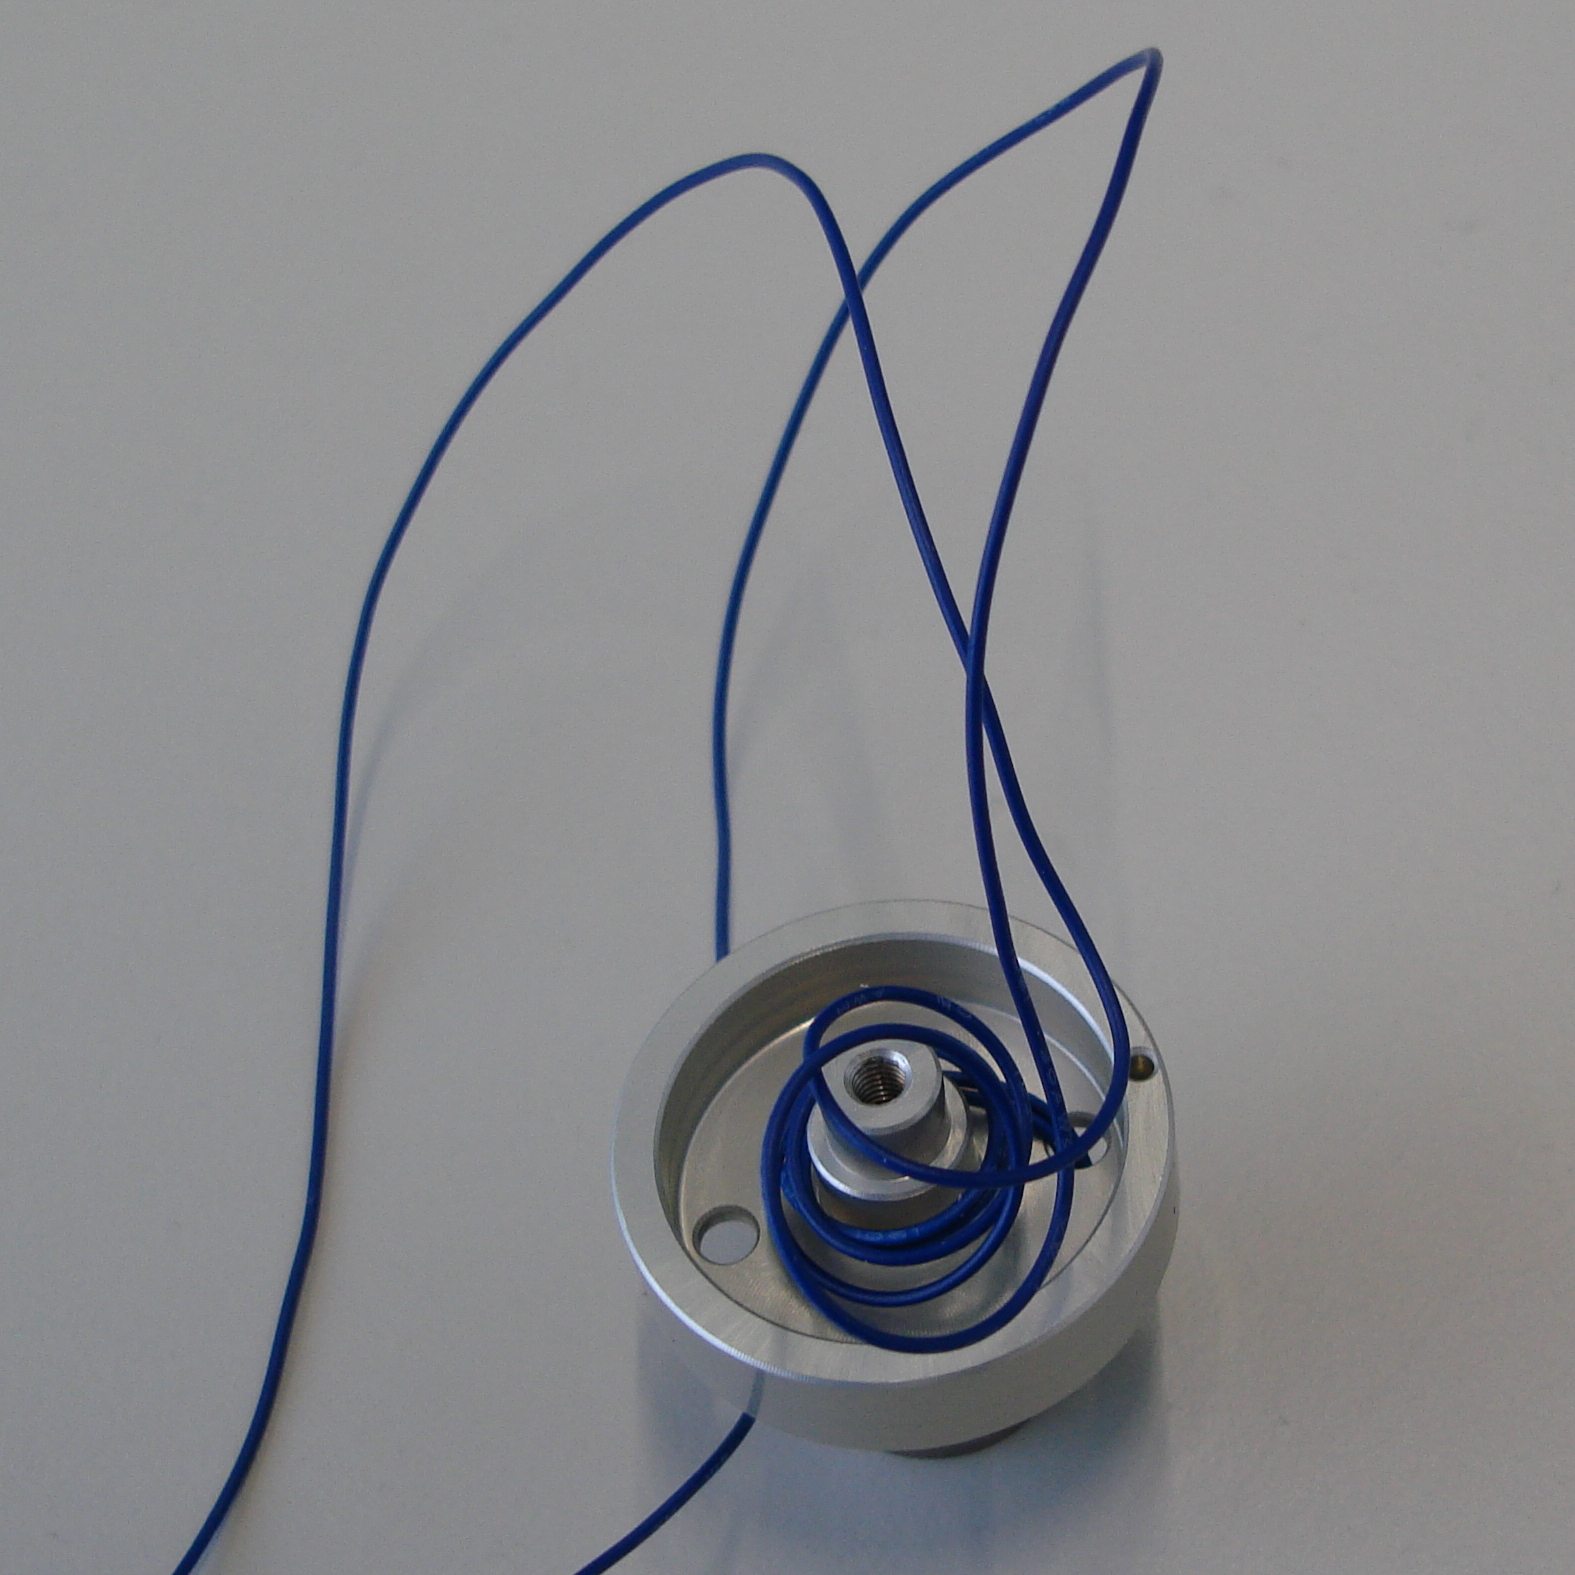
\includegraphics[width=\textwidth]{mechanicalAssemblyStep01}
	\label{fig:MechanicalAssebmlyStep01}
\end{minipage}

\subsection*{Step 2}

\begin{minipage}[t]{0.6\textwidth}
	\begin{itemize}
		\item Put a dowel pin (25) in the TCP link (9) and one in the rotating tool carrier. Measure how much the dowel pin protrudes from the rotating tool carrier (11). If it protrudes more than 1.4 mm, please abrade it. The two dowel pins will define the mechanical limit for the rotating tool carrier.
		\item Lead the cable of magnet through the hole of the TCP link.
		\item Put a groove ball bearing (17) in the TCP link.
	\end{itemize}
\end{minipage}
\hfill
\begin{minipage}[t]{0.35\textwidth}
	\vspace{-\ht\strutbox}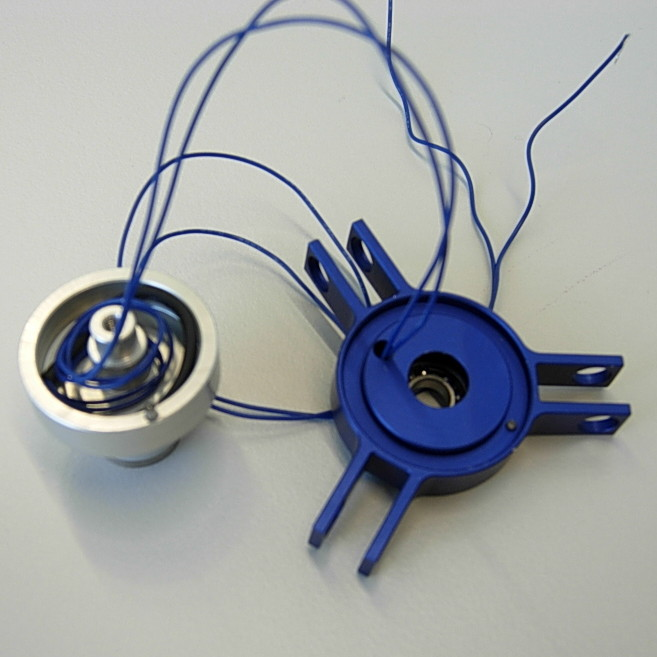
\includegraphics[width=\textwidth]{mechanicalAssemblyStep02}
	\label{fig:MechanicalAssebmlyStep02} 
\end{minipage}

\subsection*{Step 3}

\begin{minipage}[t]{0.6\textwidth}
	\begin{itemize}
		\item Link the rotating tool carrier with the TCP link on the groove ball bearing.
		\item If the connection is severe, use a vise to use the TCP motor carrier (10) as a mounting aid. Mount everything together, setting the mechanical limit so that when the rotating tool carrier turns, the cables are not stretching or tangling.
	\end{itemize}
\end{minipage}
\hfill
\begin{minipage}[t]{0.35\textwidth}
	\vspace{-\ht\strutbox}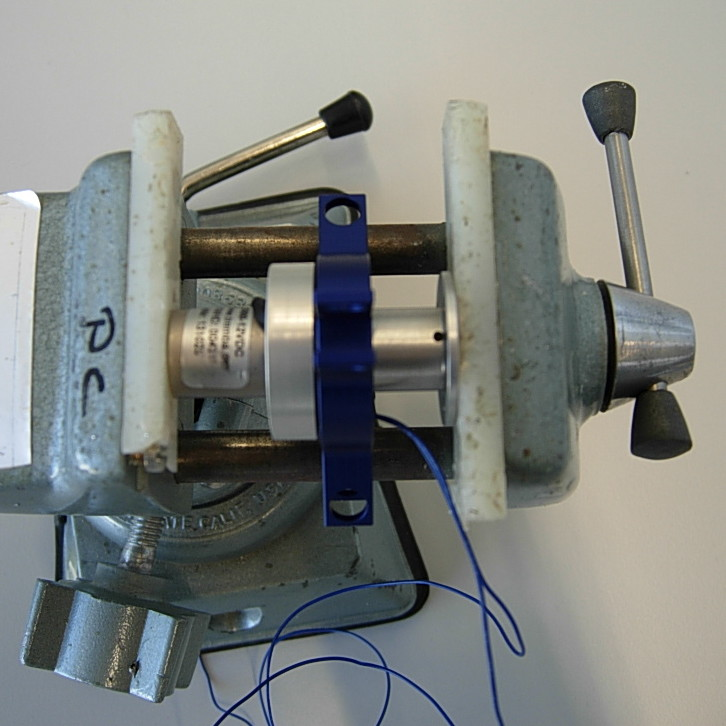
\includegraphics[width=\textwidth]{mechanicalAssemblyStep03}
	\label{fig:MechanicalAssebmlyStep03} 
\end{minipage}

\subsection*{Step 4}

\begin{minipage}[t]{0.6\textwidth}
	\begin{itemize}
		\item Put a second groove ball bearing (17) in the TCP link.
		\item Screw the tool carrier motor adapter (12) in.
		\item Screw two grub screws (19) in the tool carrier motor adapter, but not too deep.
	\end{itemize}
\end{minipage}
\hfill
\begin{minipage}[t]{0.35\textwidth}
	\vspace{-\ht\strutbox}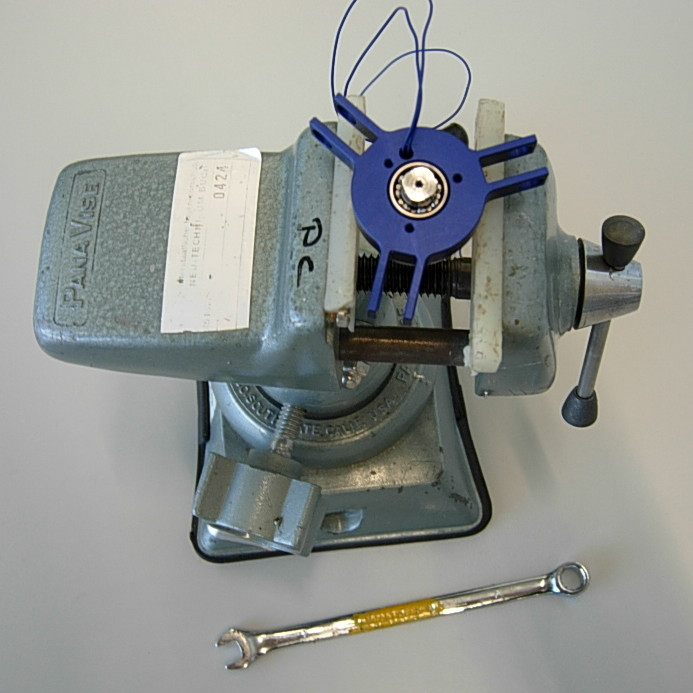
\includegraphics[width=\textwidth]{mechanicalAssemblyStep04}
	\label{fig:MechanicalAssebmlyStep04} 
\end{minipage}

\subsection*{Step 5}

\begin{minipage}[t]{0.6\textwidth}
	\begin{itemize}
		\item Mount the motor (15) on the motor carrier (10) using the cheese screws M1.2x3 (24).
		\item Lead the cable of the magnet through the hole in the motor carrier.
	\end{itemize}
\end{minipage}
\hfill
\begin{minipage}[t]{0.35\textwidth}
	\vspace{-\ht\strutbox}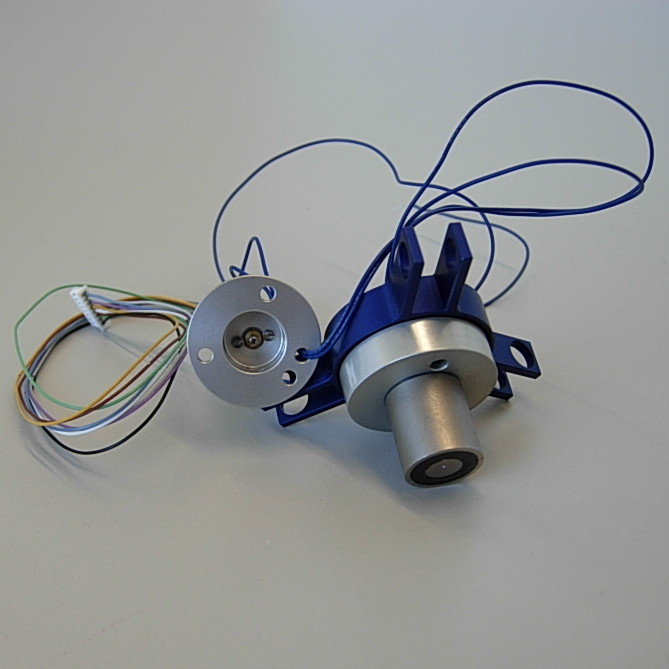
\includegraphics[width=\textwidth]{mechanicalAssemblyStep05}
	\label{fig:MechanicalAssebmlyStep05} 
\end{minipage}

\subsection*{Step 6}

\begin{minipage}[t]{0.6\textwidth}
	\begin{itemize}
		\item Mount the motor carrier (10) with the cylinder head screw M2x5 (21) on the TCP link (9). 
		\item Attach the motor shaft (15) to the tool carrier motor adapter (12) by screwing the two grub screws mounted in the tool carier on step 4.
	\end{itemize}
\end{minipage}
\hfill
\begin{minipage}[t]{0.35\textwidth}
	\vspace{-\ht\strutbox}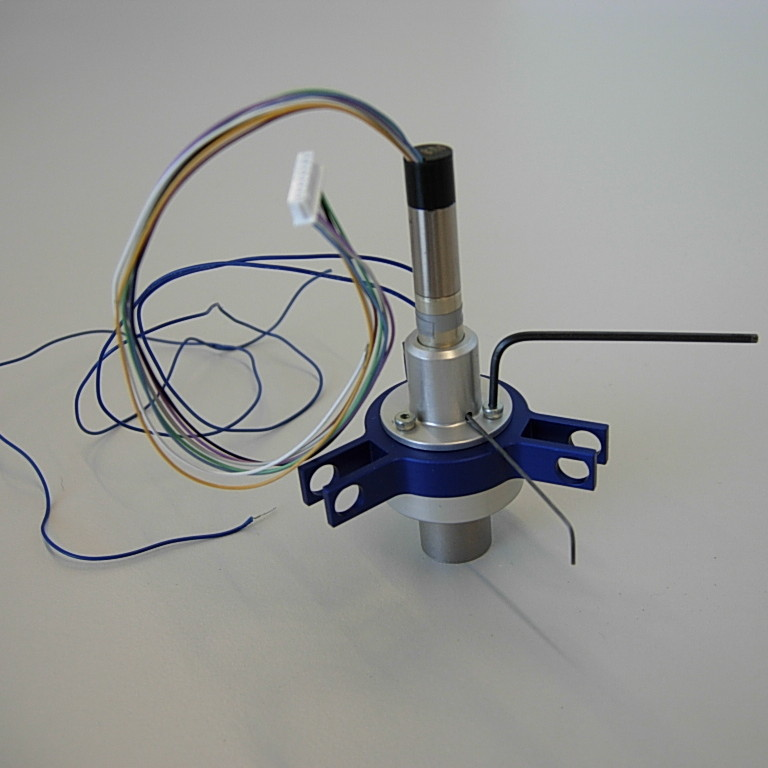
\includegraphics[width=\textwidth]{mechanicalAssemblyStep06}
	\label{fig:MechanicalAssebmlyStep06} 
\end{minipage}

\subsection*{Step 7}

\begin{minipage}[t]{0.6\textwidth}
	\begin{itemize}
		\item Fix the cable of the magnet with a cable tie.
	\end{itemize}
\end{minipage}
\hfill
\begin{minipage}[t]{0.35\textwidth}
	\vspace{-\ht\strutbox}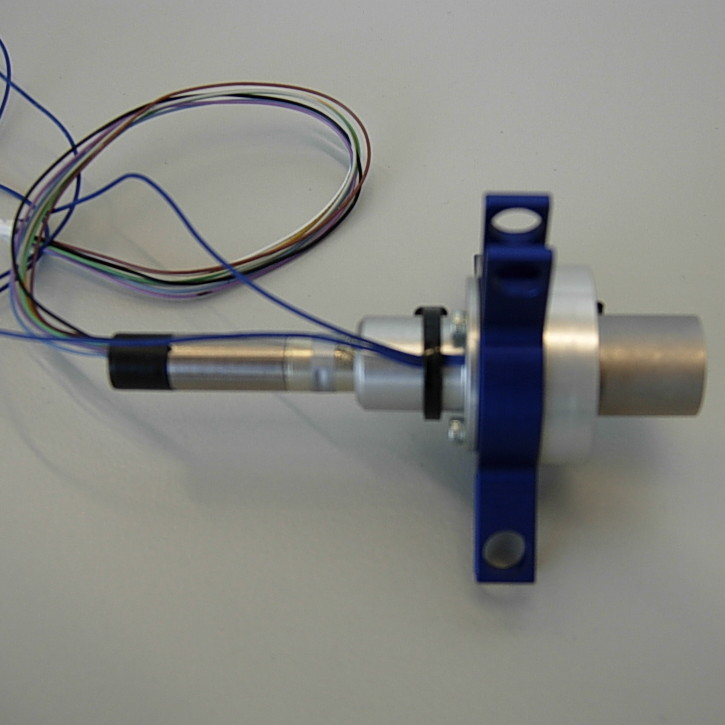
\includegraphics[width=\textwidth]{mechanicalAssemblyStep07}
	\label{fig:MechanicalAssebmlyStep07} 
\end{minipage}

\subsection*{Step 8}

\begin{minipage}[t]{0.6\textwidth}
	\begin{itemize}
		\item Mount one threaded rod (6) with four distance sleeve (4) and two ball bearing (18) together.
	\end{itemize}
\end{minipage}
\hfill
\begin{minipage}[t]{0.35\textwidth}
	\vspace{-\ht\strutbox}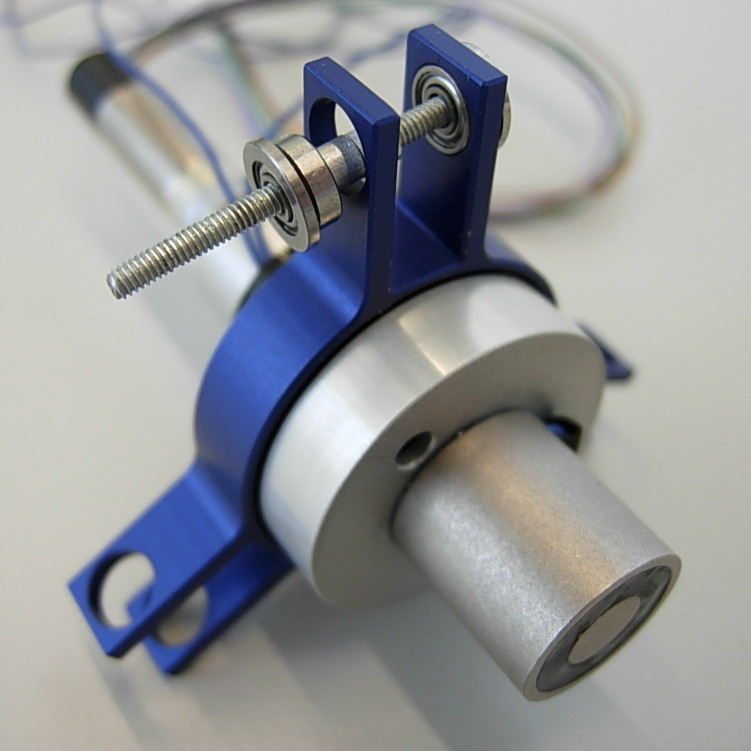
\includegraphics[width=\textwidth]{mechanicalAssemblyStep08}
	\label{fig:MechanicalAssebmlyStep08} 
\end{minipage}

\subsection*{Step 9}

\begin{minipage}[t]{0.6\textwidth}
	\begin{itemize}
		\item Screw on both ends of the threaded rod a quicklink (13).
		\item Complete this step for all three joints.
	\end{itemize}
\end{minipage}
\hfill
\begin{minipage}[t]{0.35\textwidth}
	\vspace{-\ht\strutbox}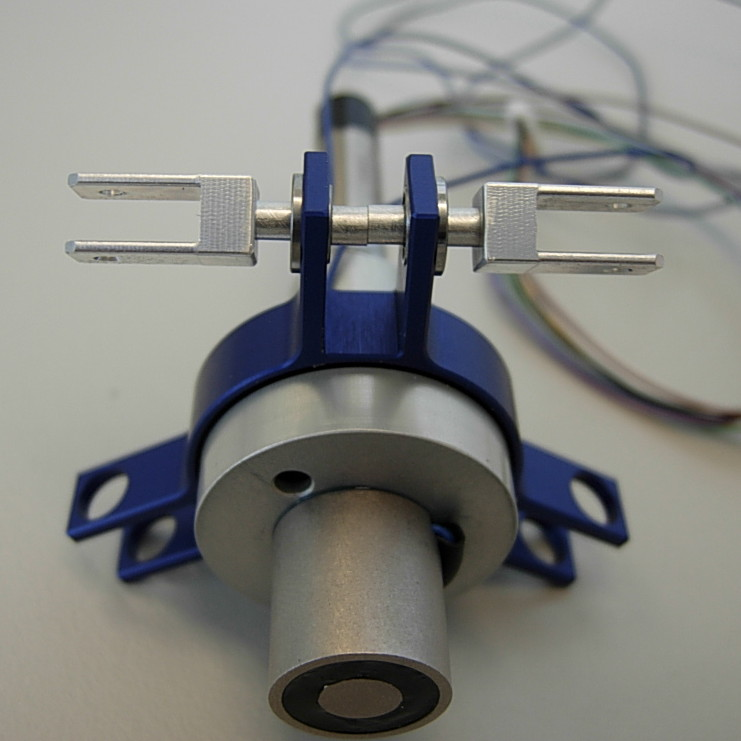
\includegraphics[width=\textwidth]{mechanicalAssemblyStep09}
	\label{fig:MechanicalAssebmlyStep09} 
\end{minipage}

\subsection*{Step 10}

\begin{minipage}[t]{0.6\textwidth}
	\begin{itemize}
		\item Repeat steps 8 and 9 also on the delta upper arms (3).
		\item Screw two grub screws M3x3 (xxx) in the Delta upper arms (3), but not too deep.
	\end{itemize}
\end{minipage}
\hfill
\begin{minipage}[t]{0.35\textwidth}
	\vspace{-\ht\strutbox}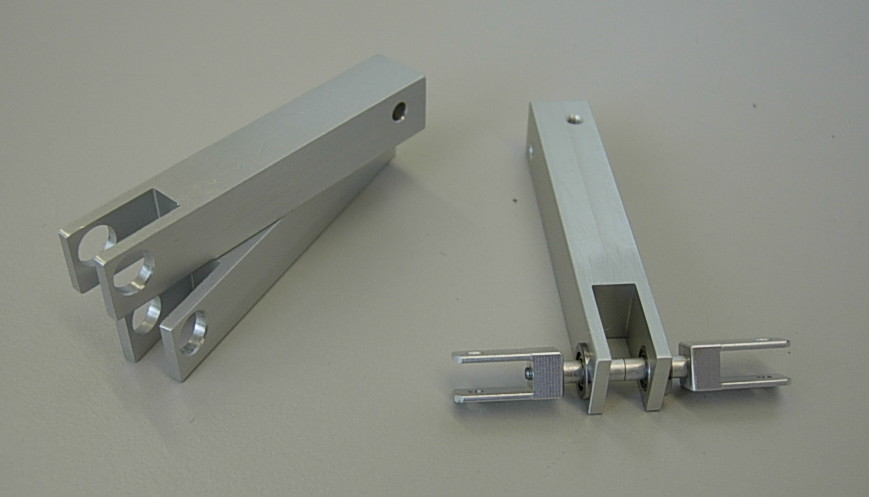
\includegraphics[width=\textwidth]{mechanicalAssemblyStep10}
	\label{fig:MechanicalAssebmlyStep10} 
\end{minipage}

\subsection*{Step 11}

\begin{minipage}[t]{0.6\textwidth}
	\begin{itemize}
		\item The arms can be built using two nuts (23), a thread rod (7), a carbon tube (5) and two Igubal rod end spherical bearings (16).
		\item Make six arms.
	\end{itemize}
\end{minipage}
\hfill
\begin{minipage}[t]{0.35\textwidth}
	\vspace{-\ht\strutbox}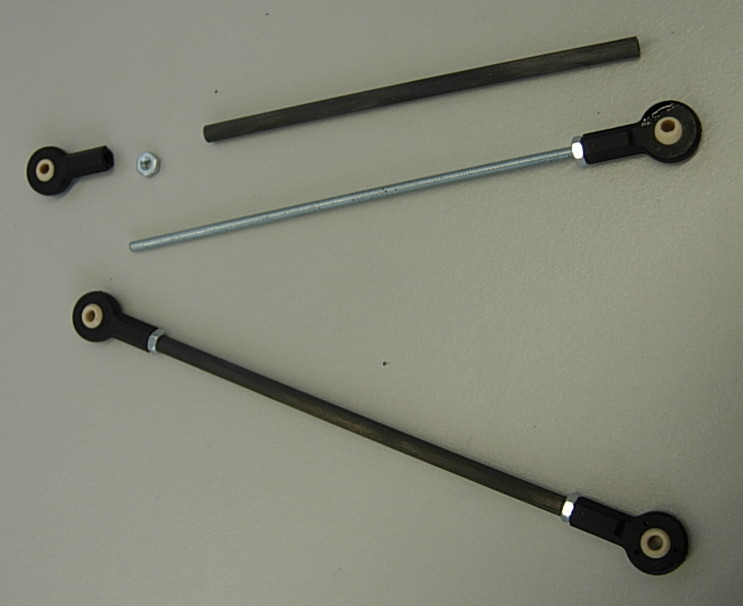
\includegraphics[width=\textwidth]{mechanicalAssemblyStep11}
	\label{fig:MechanicalAssebmlyStep11} 
\end{minipage}

\subsection*{Step 12}

\begin{minipage}[t]{0.6\textwidth}
	\begin{itemize}
		\item Attach the motor (14) on the delta motor carrier (2) with two cylinder head screws M2x4 (xxx). Screw the two grub screws mounted on step 10 on the delta upper arms. Important: the grub screws have to press on the straight surface of the motor shaft.
	\end{itemize}
\end{minipage}
\hfill
\begin{minipage}[t]{0.35\textwidth}
	\vspace{-\ht\strutbox}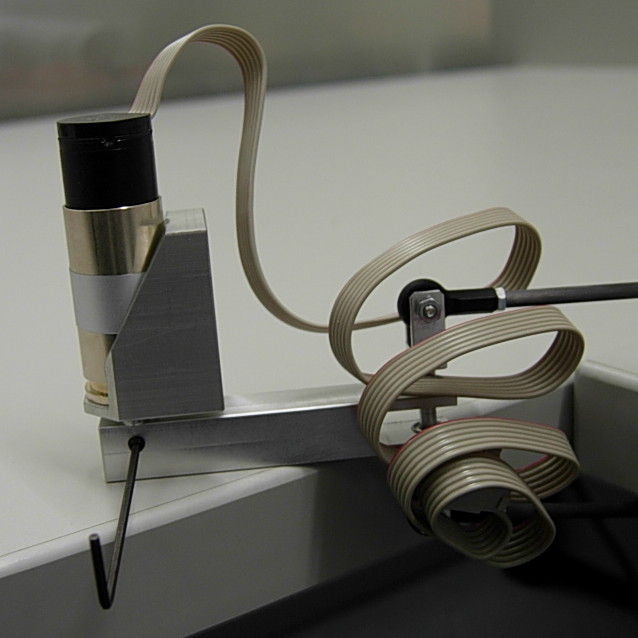
\includegraphics[width=\textwidth]{mechanicalAssemblyStep12}
	\label{fig:MechanicalAssebmlyStep12} 
\end{minipage}

\subsection*{Step 13}

\begin{minipage}[t]{0.6\textwidth}
	\begin{itemize}
		\item Mount the three delta motor carrier (2) on the delta top carrier (1), note that the orientation of the motors must be counter clockwise.
	\end{itemize}
\end{minipage}
\hfill
\begin{minipage}[t]{0.35\textwidth}
	\vspace{-\ht\strutbox}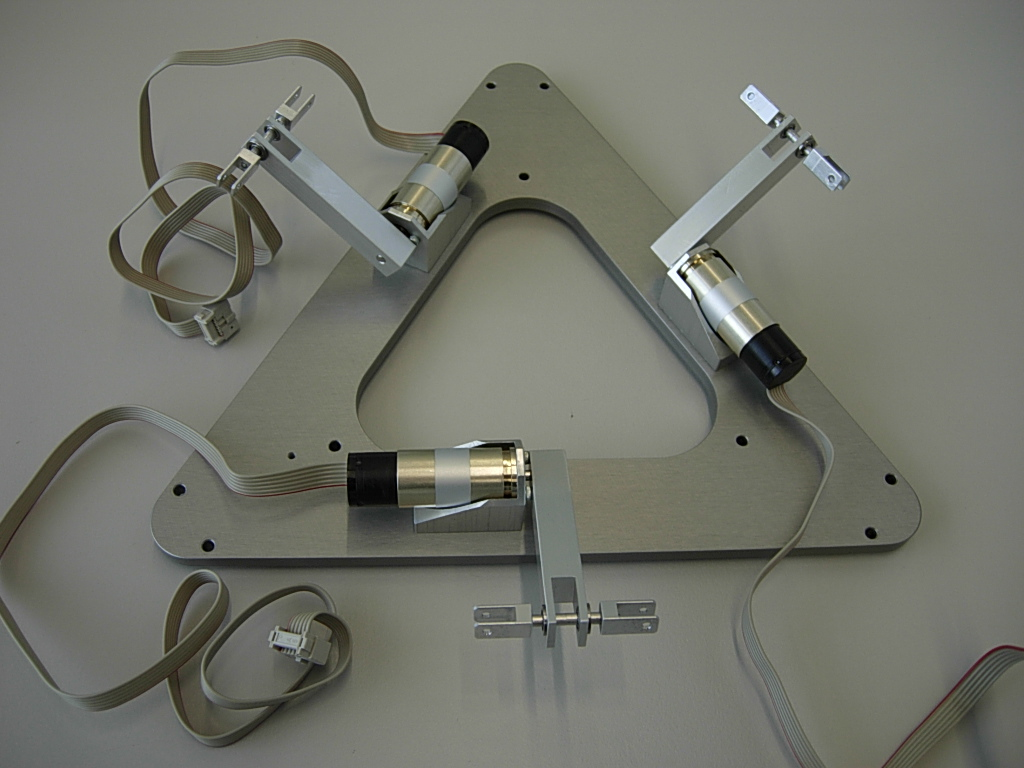
\includegraphics[width=\textwidth]{mechanicalAssemblyStep13}
	\label{fig:MechanicalAssebmlyStep13} 
\end{minipage}

\subsection*{Step 14}

\begin{minipage}[t]{0.6\textwidth}
	\begin{itemize}
		\item Connect the TCP link (9) to the delta upper arms (3) through the arms that were built at step 11, using the cylinder screws M2x8 (22) and nuts (23).
		\item The image gives an overview of the whole construction. Please ignore the orientation of the motors in this image, since it is not the same as for your robot.
	\end{itemize}
\end{minipage}
\hfill
\begin{minipage}[t]{0.35\textwidth}
	\vspace{-\ht\strutbox}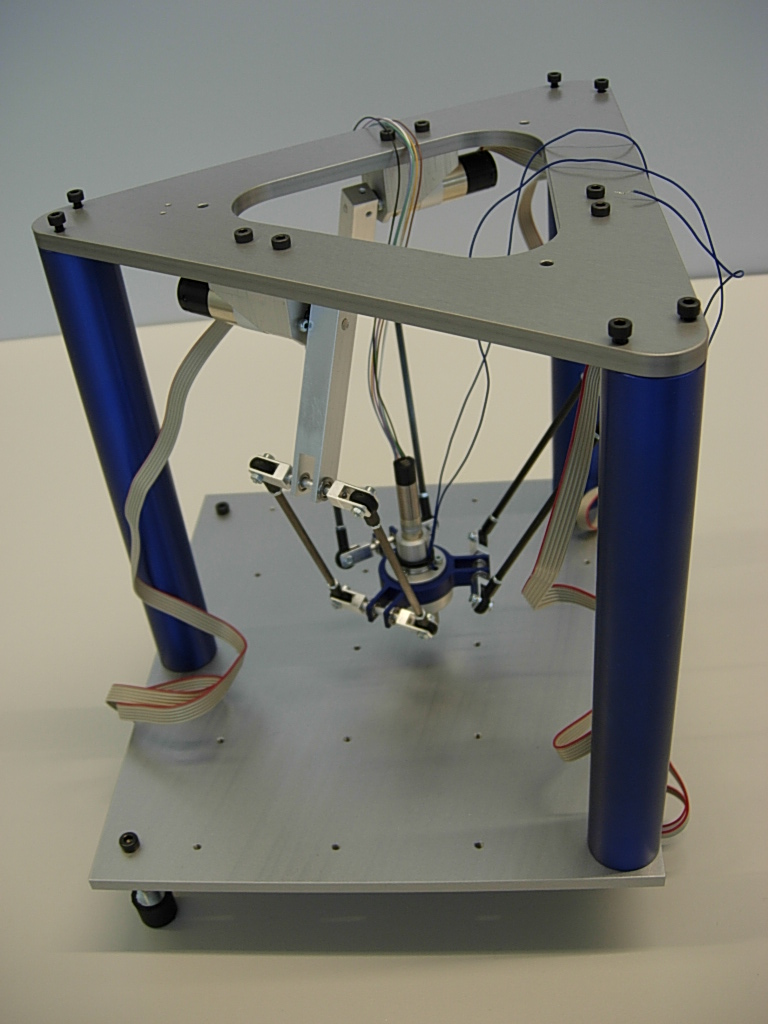
\includegraphics[width=\textwidth]{mechanicalAssemblyStep14}
	TODO: replace Image
	\label{fig:MechanicalAssebmlyStep14} 
\end{minipage}

\section{Base Case}
TODO Stefan

\section{Remote Case}
TODO Stefan

\section{Tile playing field}
TODO Stefan

\chapter{PCB assembly}
\section{Main board}
TODO Martin

\section{HMI extension board}

The HMI extension board connects three buttons with integrated LEDs to the FPGA on the main board. For connecting both boards, a 20 wire ribbon cable is used (see Appendix \ref{sec:hmiExtensionCables} at page \ref{sec:hmiExtensionCables} for detailed information about the cable). This cable connects P1 on the main board with P1 on the extension board.

The buttons are connected with 4 wire ribbon cables as described in appendix \ref{sec:hmiExtensionCables}. Use U1 to connect the blue button, U2 for the red and U3 for the green.

\begin{figure}[htbp]
	\centering
	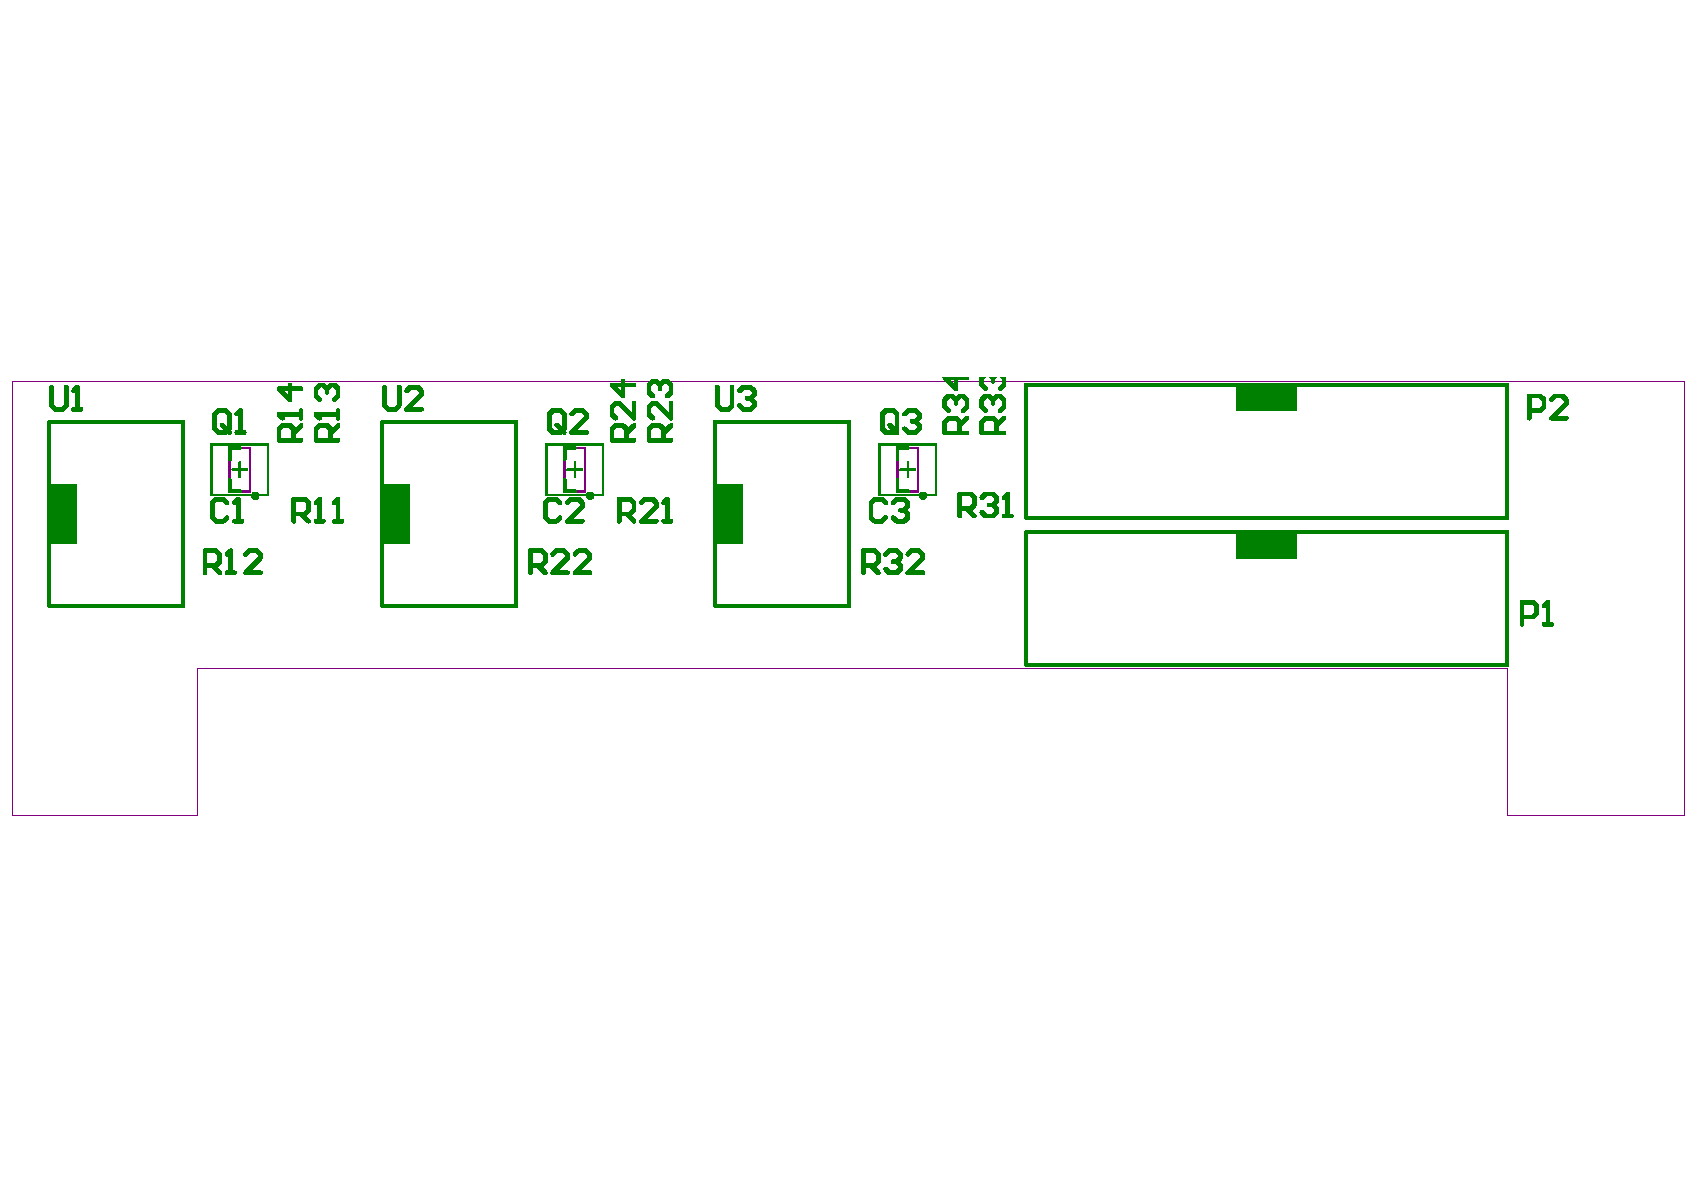
\includegraphics[width=\textwidth]{EeduroHmiExtensionAssembly}
	\caption{EEDURO HMI extension board assembly drawing}
	\label{fig:EeduroHmiExtensionAssembly}
\end{figure}

On the EEDURO main board Revision 3 or older, a reset circuit for the FPGA is missing. As a workaround this can be assembled instead of P2 on the extension board. There is also no support voltage available on P1 of the main board. Therefore a two way Molex connector P6 is used. Figure \ref{fig:EeduroHmiExtensionP2Replacement} shows the necessary modification.

\begin{figure}[htbp]
	\centering
	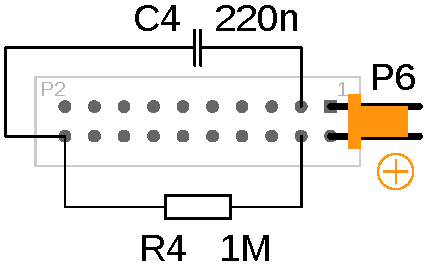
\includegraphics[width=0.5\textwidth]{EeduroHmiExtensionP2Replacement}
	\caption{EEDURO HMI extension board modifications}
	\label{fig:EeduroHmiExtensionP2Replacement}
\end{figure}

\section{Line receiver board}

\section{Line transmitter board}

\chapter{Wiring}
\section{Delta robot with base case}
TODO

\section{Delta robot with remote case}

\begin{figure}[htbp]
	\centering
	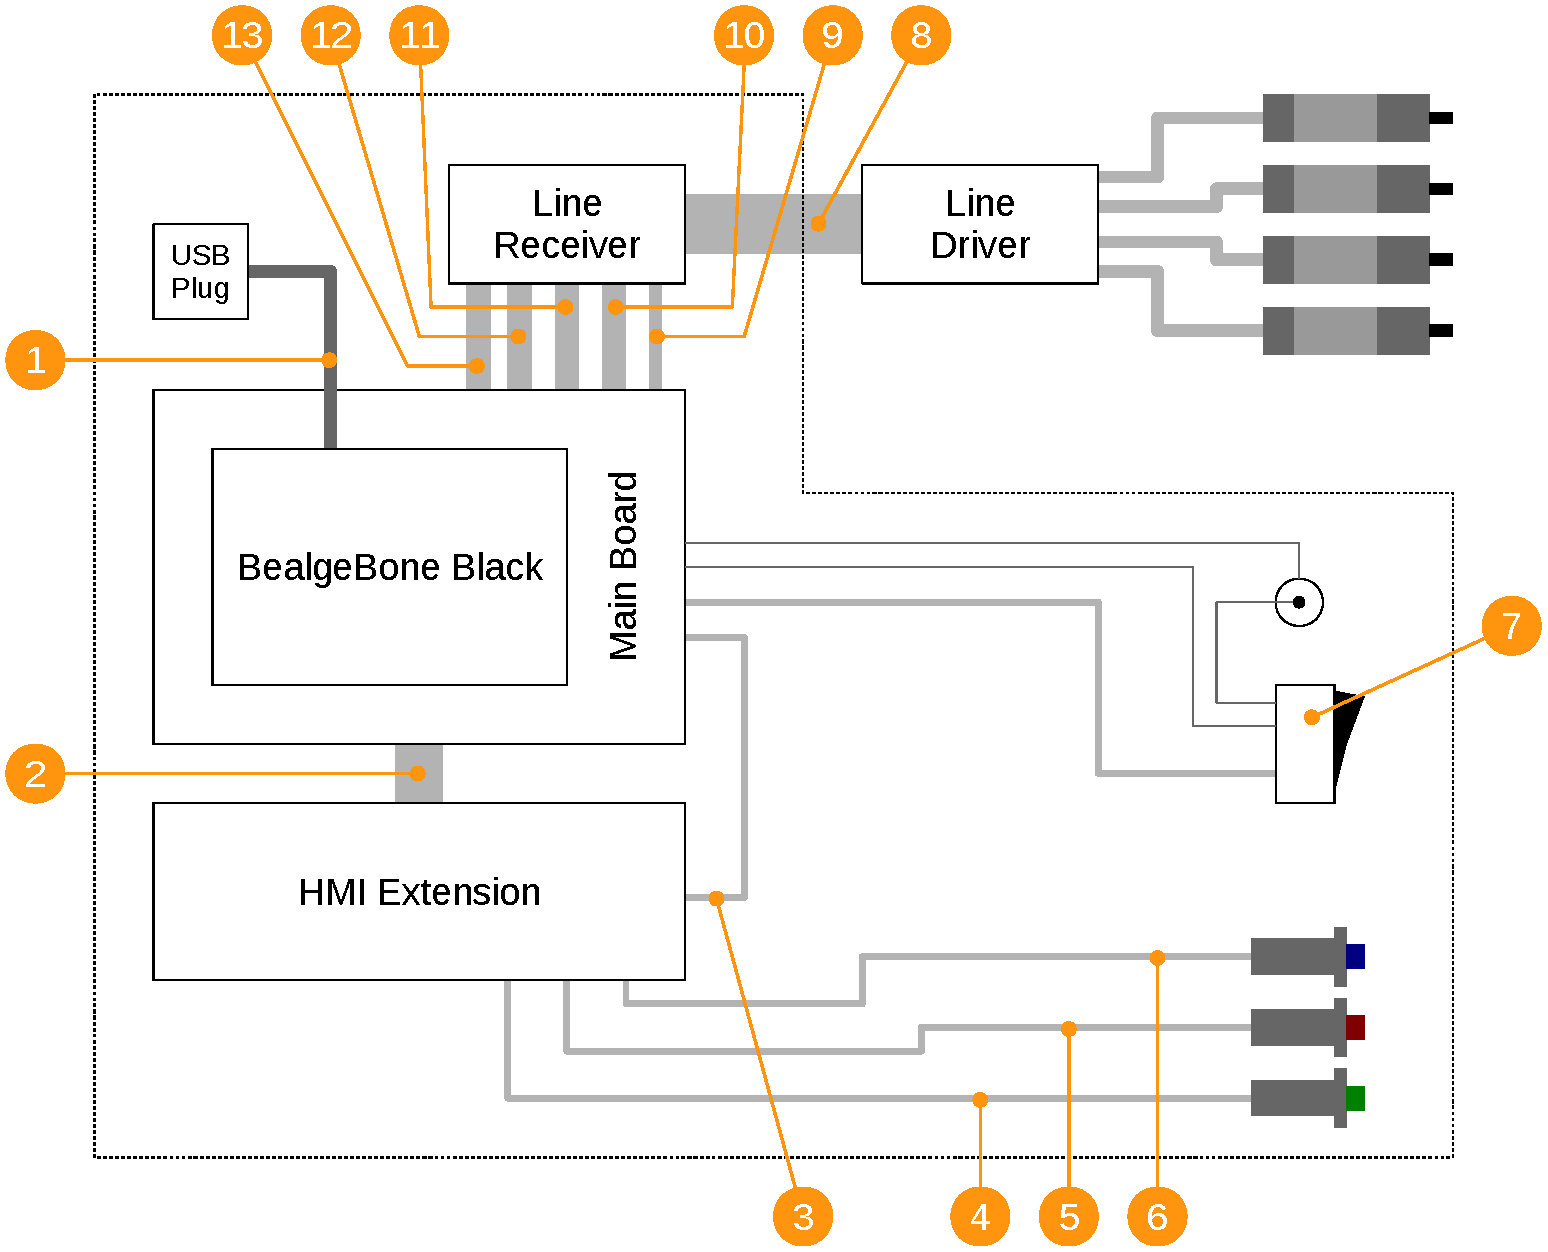
\includegraphics[width=\textwidth]{CablingOverviewRemoteCase}
	\caption{Cabling overview for the EEDURO delta robot with a remote control case}
	\label{fig:CablingOverviewRemoteCase}
\end{figure}

Build instructions for the cables can be found in appendix \ref{sec:cableBuildInstructions} on page \pageref{sec:cableBuildInstructions}.

\begin{enumerate}[(1)]
	\item USB extension cable with panel jack, see part list in appendix \ref{sec:bom-remotecase} at page \pageref{sec:bom-remotecase}. Connect to \textit{USB Host} (\texttt{P3}) on the BeagleBone Black.
	\item 20 wire ribbon cable, connects \texttt{P1} on the main board with \texttt{P1} on the HMI extension board. 
	\item HMI extension board power cable. Connects \texttt{P6} on the extension board to the power terminal \texttt{P2} on the main board. Consider the polarity!
	\item Green button with integrated LED for user interaction. Connect to \texttt{U3} on the HMI extension board.
	\item Red button with integrated LED for user interaction. Connect to \texttt{U2} on the HMI extension board.
	\item Blue button with integrated LED for user interaction. Connect to \texttt{U1} on the HMI extension board.
	\item Connect the black ground wire (coming from the power connector \texttt{X5}) and the red wire (coming from the power switch) to the terminal \texttt{P2} on the main board. Also connect the two wire cable for the power LED to the \texttt{P2} terminal.
	\item 34 way ribbon cable to the robot. Use \texttt{X4} of the remote case.
	\item 4 way ribbon cable for the electro magnet (Position 28 in Figure \ref{fig:DeltaMechanicalPartsOverviewTCP} at page \pageref{fig:DeltaMechanicalPartsOverviewTCP}) and the supply voltage for the line receiver board. Connect \texttt{P1} on the line receiver board with \texttt{POUT} on the mainboard.
	\item 6 way ribbon cable for axis 1 (Motor 0). Connect \texttt{MOT1} on the line receiver board with \texttt{MOTOR0} on the mainboard.
	\item 6 way ribbon cable for axis 2 (Motor 1). Connect \texttt{MOT2} on the line receiver board with \texttt{MOTOR1} on the mainboard.
	\item 6 way ribbon cable for axis 3 (Motor 2). Connect \texttt{MOT3} on the line receiver board with \texttt{MOTOR2} on the mainboard.
	\item 6 way ribbon cable for axis 4 (Motor 3). Connect \texttt{MOT4} on the line receiver board with \texttt{MOTOR3} on the mainboard.
\end{enumerate}

A full wired remote case is shown in figure \ref{fig:RemoteCaseOpenWithBBB} on page \pageref{fig:RemoteCaseOpenWithBBB}.

\chapter{Testing}
TODO

\appendix
\addchap{\appendixname}
\makeatletter
	\@addtoreset{figure}{section}
	\@addtoreset{table}{section}
\makeatother\renewcommand{\thefigure}{\Alph{section}.\arabic{figure}}
\renewcommand{\thetable}{\Alph{section}.\arabic{table}}
\renewcommand{\thesection}{\Alph{section}}

\section{Part list}
\label{sec:bom}

\subsection{Overview}

\begin{tabular}{m{5cm} m{7cm} m{2cm}}
\hline
EEDURO Delta Robot          & sub parts see appendix \ref{sec:bom-robot} at page \pageref{sec:bom-robot}           & 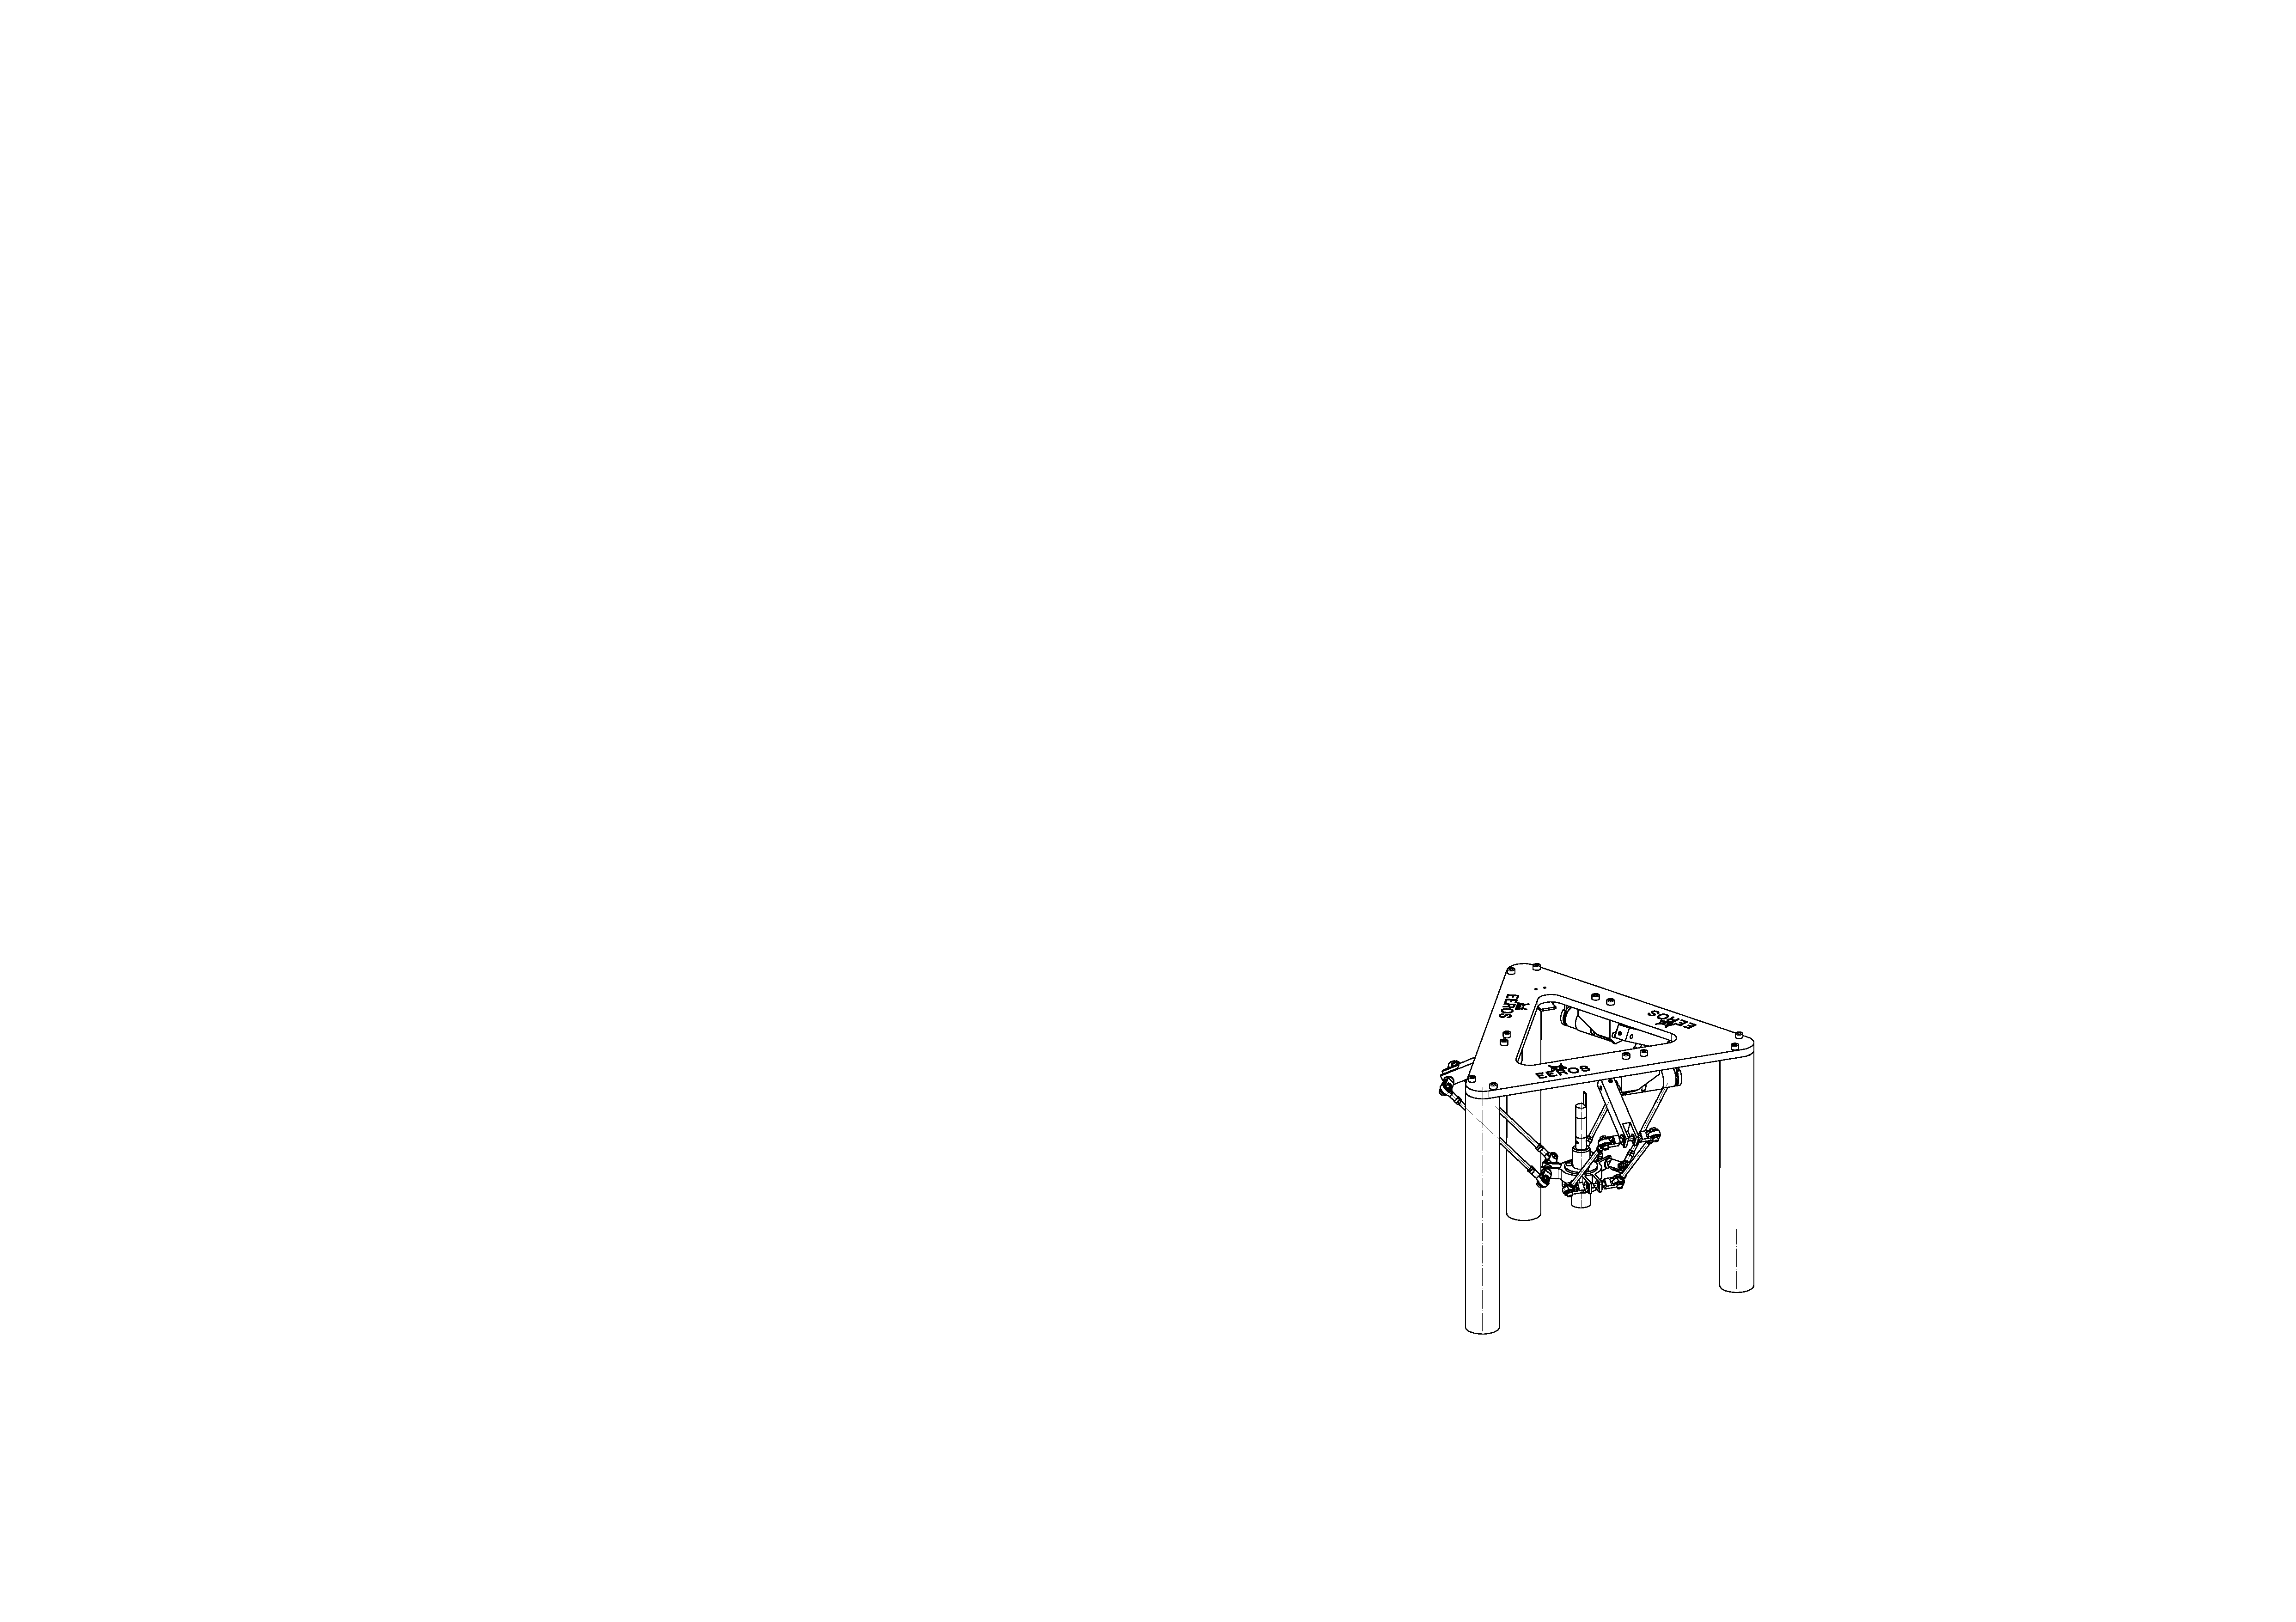
\includegraphics[height=2cm]{EeduroDeltaRobotOnly} \\
\hline
EEDURO Base case            & sub parts see appendix \ref{sec:bom-basecase} at page \pageref{sec:bom-basecase}     & 
\includegraphics[height=2cm]{bom_blank}            \\
\hline
EEDURO Remote Case          & sub parts see appendix \ref{sec:bom-remotecase} at page \pageref{sec:bom-remotecase} & 
\includegraphics[height=2cm]{bom_blank}            \\
\hline
EEDURO Tile Play Set        & sub parts see appendix \ref{sec:bom-tileset} at page \pageref{sec:bom-tileset}       & 
\includegraphics[height=2cm]{bom_blank}            \\
\hline
EEDURO Delta Pencil Tool    & sub parts see appendix \ref{sec:bom-pencilset} at page \pageref{sec:bom-pencilset}   & 
\includegraphics[height=2cm]{bom_blank}            \\
\hline
\end{tabular}

\subsection{EEDURO Delta Robot}
\label{sec:bom-robot}

\begin{tabular}{m{0.5cm} m{5cm} m{5cm} m{1cm} m{1.5cm}}
\bfseries Qty & \bfseries Description               & \bfseries Details                &                                                   & \bfseries Reference \\
\hline
1    & Delta top carrier                            & Drawing \texttt{EEDURO-D-001}    & 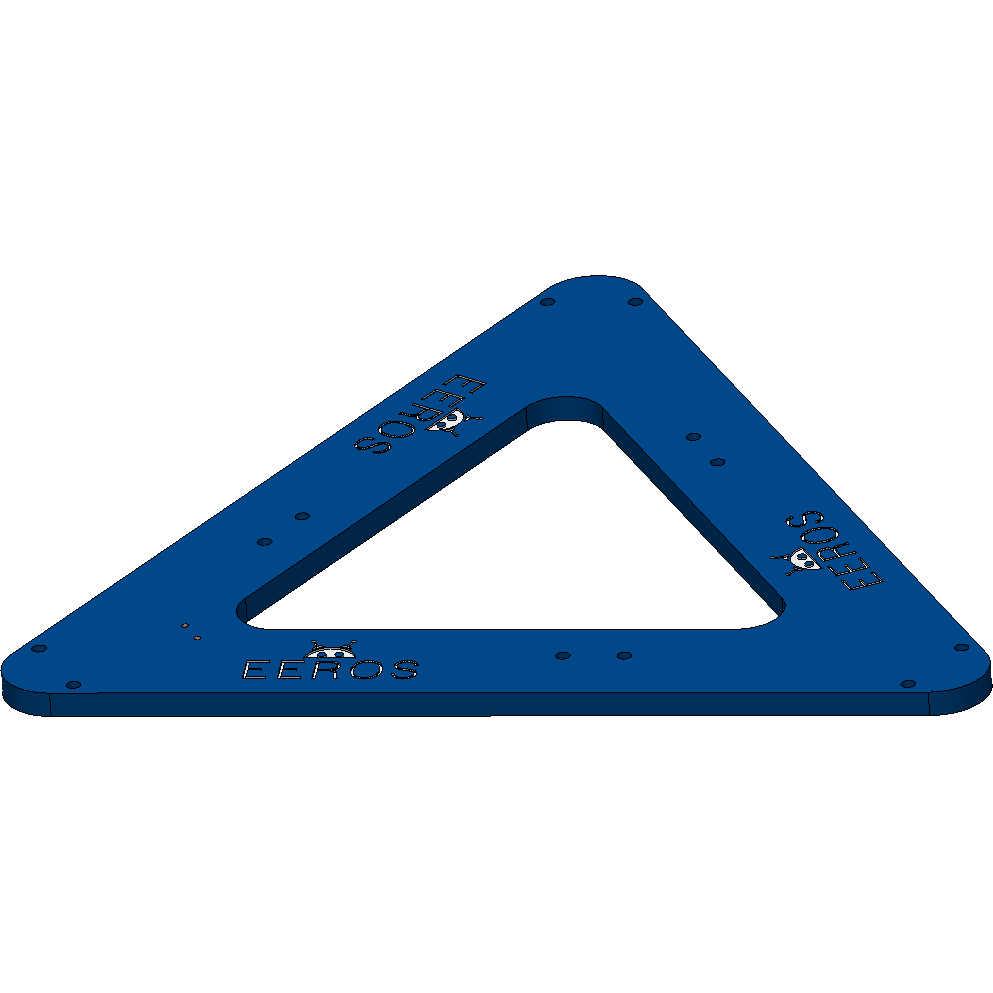
\includegraphics[height=1cm]{bom_d-001}           & 1    \\
\hline
3    & Delta motor carrier                          & Drawing \texttt{EEDURO-D-002}    & 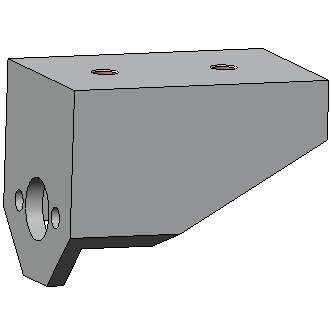
\includegraphics[height=1cm]{bom_d-002}           & 2    \\
\hline
3    & Delta upper arm                              & Drawing \texttt{EEDURO-D-003}    & 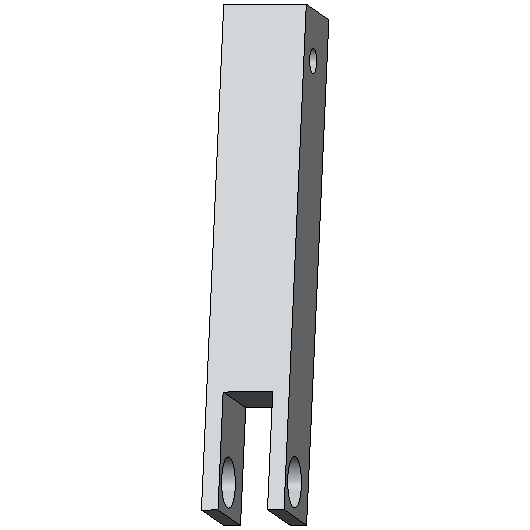
\includegraphics[height=1cm]{bom_d-003}           & 3    \\
\hline
24   & Distance sleeve ($\varnothing 2/3\times2.8$) & Drawing \texttt{EEDURO-D-004}    & 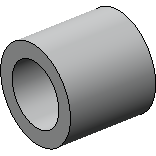
\includegraphics[height=1cm]{bom_d-004}           & 4    \\
\hline
6    & Carbon tube ($\varnothing 2/3\times72$)      & Drawing \texttt{EEDURO-D-005}    & 
\includegraphics[height=1cm]{bom_d-005}           & 5    \\
\hline
6    & Threaded rod ($M2\times25$)                  & Drawing \texttt{EEDURO-D-006}    & 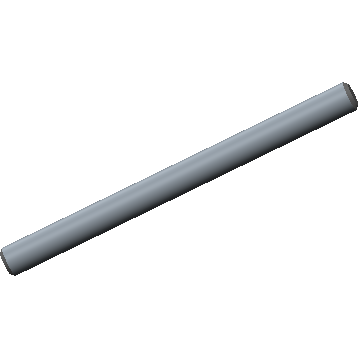
\includegraphics[height=1cm]{bom_d-006}           & 6    \\
\hline
6    & Threaded rod ($M2\times85$)                  & Drawing \texttt{EEDURO-D-007}    & 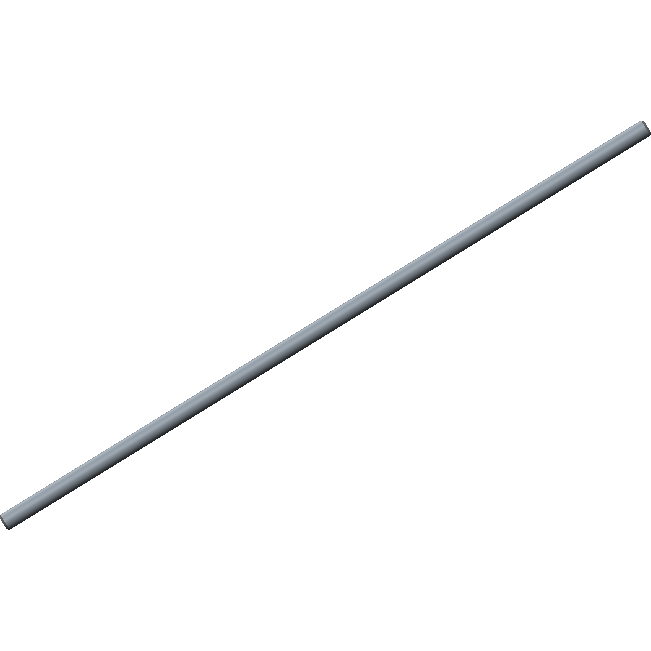
\includegraphics[height=1cm]{bom_d-007}           & 7    \\
\hline
3    & Pillar                                       & Drawing \texttt{EEDURO-D-008}    & 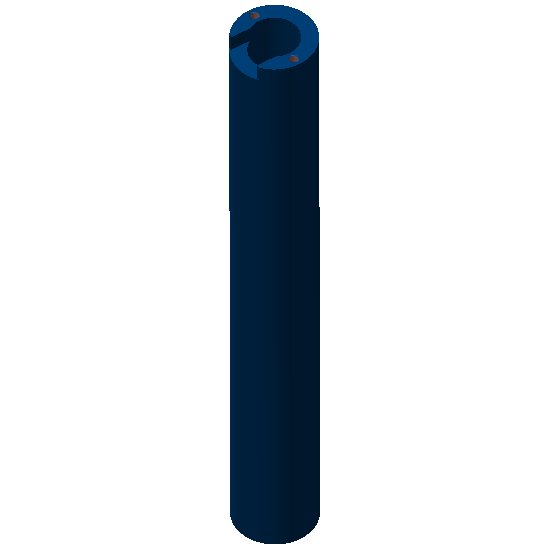
\includegraphics[height=1cm]{bom_d-008}           & 8    \\
\hline
1    & TCP link                                     & Drawing \texttt{EEDURO-D-009}    & 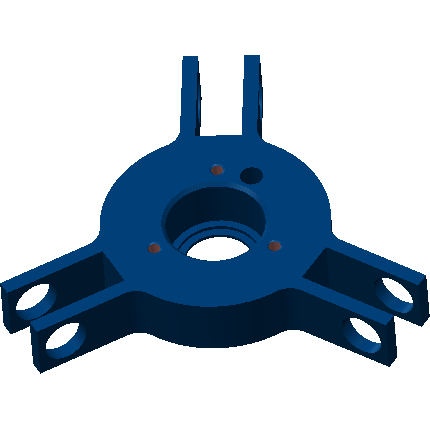
\includegraphics[height=1cm]{bom_d-009}           & 9    \\
\hline
1    & TCP motor carrier                            & Drawing \texttt{EEDURO-D-010}    & 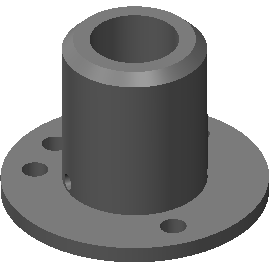
\includegraphics[height=1cm]{bom_d-010}           & 10    \\
\hline
1    & Rotating tool carrier                        & Drawing \texttt{EEDURO-D-011}    & 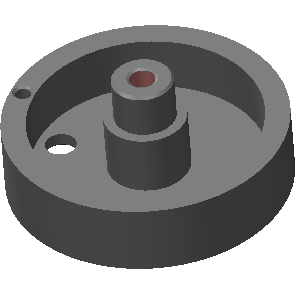
\includegraphics[height=1cm]{bom_d-011}           & 11    \\
\hline
1    & Tool carrier motor adapter                   & Drawing \texttt{EEDURO-D-012}    & 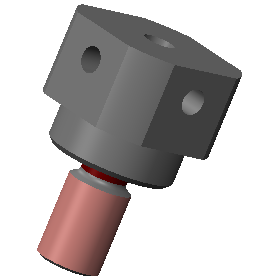
\includegraphics[height=1cm]{bom_d-012}           & 12    \\
\hline
12   & Quicklink                                    & Drawing \texttt{EEDURO-D-013}    & 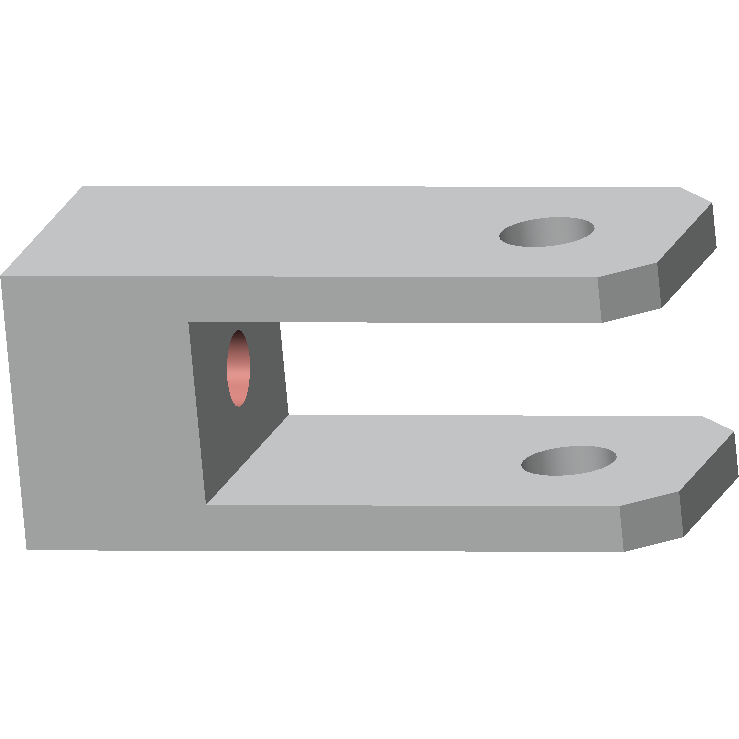
\includegraphics[height=1cm]{bom_d-013}           & 13    \\
\hline
3    & Faulhaber DC-Motor with gear                 & 1524E012SR + IEH2-4096 + 15/8-76:1 & 
\includegraphics[height=1cm]{bom_blank}         & 14    \\
\hline
1    & Faulhaber DC-Motor with gear                 & 0816D012SR-K256 \mbox{+ HEM3-256-W} + 08/3-120:1 & 
\includegraphics[height=1cm]{bom_blank} & 15 \\
\hline
12   & Igubal rod end spherical bearing             & Igus KBRM-02                     & 
\includegraphics[height=1cm]{bom_blank}           & 16    \\
\hline
2    & Groove ball bearing 16/6x3.5                 & Type 686                         & 
\includegraphics[height=1cm]{bom_blank}           & 17    \\
\hline
12   & Ball bearing F692ZZ                          & Type F692ZZ                      & 
\includegraphics[height=1cm]{bom_blank}           & 18    \\
\hline
\end{tabular}

\begin{tabular}{m{0.5cm} m{5cm} m{5cm} m{1cm} m{1.5cm}}
\bfseries Qty & \bfseries Description               & \bfseries Details             &                                                   & \bfseries Reference\\
\hline
2    & Grub screw M1.6x3                            &                               & 
\includegraphics[height=1cm]{bom_blank}           & 19    \\
\hline
12   & Cylinder head screw M3x10                    & ISO 4762                      & 
\includegraphics[height=1cm]{bom_blank}           & 20    \\
\hline
3    & Cylinder head screw M2x5                     & ISO 4762                      & 
\includegraphics[height=1cm]{bom_blank}           & 21    \\
\hline
12   & Cylinder head screw M2x8                     & ISO 4762                      & 
\includegraphics[height=1cm]{bom_blank}           & 22    \\
\hline
24   & Nut M2                                       & ISO 4032                      & 
\includegraphics[height=1cm]{bom_blank}           & 23    \\
\hline
2    & Cheese screw M1.2x3                          &                               & 
\includegraphics[height=1cm]{bom_blank}           & 24    \\
\hline
2    & Dowel pin $\varnothing 1.5\times5h6$         &                               & 
\includegraphics[height=1cm]{bom_blank}           & 25    \\
\hline
6    & Grub screw M2.5x3                            &                               & \includegraphics[height=1cm]{bom_blank}           & 26    \\
\hline
6    & Cylinder head screw M2x4                     & ISO 4762                      & \includegraphics[height=1cm]{bom_blank}           & 27    \\
\hline
1    & Electro magnet                               & Tremba GTO-14-0.5000          & \includegraphics[height=1cm]{bom_blank}           & 28    \\
\hline
1    & Grub screw M2x8                              &                               & \includegraphics[height=1cm]{bom_blank}           & 29    \\
\hline
\end{tabular}

\subsection{Base case}
\label{sec:bom-basecase}

\begin{tabular}{m{0.5cm} m{5cm} m{5cm} m{1cm} m{1.5cm}}
\bfseries Qty  & \bfseries Description              & \bfseries Details                              &                                           & \bfseries Reference\\
\hline
1    & EEDURO base case                             & Drawing \texttt{EEDURO-001}                    & \includegraphics[height=1cm]{bom_e-001}   & 1   \\
\hline
1    & Base case cover (plexiglas)                  & Drawing \texttt{EEDURO-002}                    & \includegraphics[height=1cm]{bom_e-002}   & 2   \\
\hline
1    & EEDURO main board                            & sub parts see appendix \ref{sec:bom-mainboard} & \includegraphics[height=1cm]{bom_blank}   & 3   \\
\hline
1    & HMI extension board                          & sub parts see appendix \ref{sec:bom-hmiext}    & \includegraphics[height=1cm]{bom_blank}   & 4   \\
\hline
1    & Power connector with switch                  & sub parts see appendix \ref{sec:bom-pwr}       & \includegraphics[height=1cm]{bom_blank}   & 5   \\
\hline
1    & Power supply 12\,V, 1.5\,A                   & TBD                                            & \includegraphics[height=1cm]{bom_blank}   & 6   \\
\hline
1    & USB cable with panel jack                    & Ampire XUB060                                  & \includegraphics[height=1cm]{bom_blank}   & 7   \\
\hline
1    & USB mini extension cable                     & Length: ca. 200\,mm                            & \includegraphics[height=1cm]{bom_blank}   & 8   \\
\hline
1    & USB mini panel mount                         & Drawing \texttt{EEDURO-003}                    & \includegraphics[height=1cm]{bom_e-003}   & 9   \\
\hline
4    & Cylinderic rubber pad M3                     & Norelem 26106-00800855                         & \includegraphics[height=1cm]{bom_blank}   & 10   \\
\hline
6    & Cylinder head screw M3x12                    & ISO 4762                                       & \includegraphics[height=1cm]{bom_blank}   & 11   \\
\hline
2    & Countersunk head screw, M3x12                & ISO 10642                                      & \includegraphics[height=1cm]{bom_blank}   & 12   \\
\hline
2    & Washer M3                                    &                                                & \includegraphics[height=1cm]{bom_blank}   & 13   \\
\hline
2    & Nut M3                                       & ISO 4032                                       & \includegraphics[height=1cm]{bom_blank}   & 14   \\
\hline
\end{tabular}

\subsection{Remote case}
\label{sec:bom-remotecase}

\begin{tabular}{m{0.5cm} m{5cm} m{5cm} m{1cm} m{1.5cm}}
\bfseries Qty  & \bfseries Description              & \bfseries Details                                 &                                          & \bfseries Reference\\
\hline
1    & Remote case                                  & \mbox{Hammond 1455T2201BU}, \mbox{see Drawing \texttt{TBD}} & \includegraphics[height=1cm]{bom_remotecase} & 1    \\
\hline
1    & Main board                                   & sub parts see appendix \ref{sec:bom-mainboard}    & \includegraphics[height=1cm]{bom_blank}   & 2   \\
\hline
1    & HMI extension board                          & sub parts see appendix \ref{sec:bom-hmiext}       & \includegraphics[height=1cm]{bom_blank}   & 3   \\
\hline
1    & Line Receiver board                          & sub parts see appendix \ref{sec:bom-linerec}      & \includegraphics[height=1cm]{bom_blank}   & 4    \\
\hline
1    & Power connector with switch                  & sub parts see appendix \ref{sec:bom-pwr}       & \includegraphics[height=1cm]{bom_blank}   & 5   \\
\hline
1    & Power supply 12\,V, 1.5\,A                   & Nordic Power AM04151A-12V                         & \includegraphics[height=1cm]{bom_powersupply12V} & 6   \\
\hline
1    & USB cable with panal jack                    & Ampire XUB060                                     & \includegraphics[height=1cm]{bom_blank} & 7   \\
\hline
4    & Spacer bolt M3x5\,mm                         & Distrelec 340962                                  & \includegraphics[height=1cm]{bom_spacerbolt} & 8   \\
\hline
6    & Countersunk head screw, M3x6                 & ISO 10642                                         & \includegraphics[height=1cm]{bom_blank}   & 9   \\
\hline
4    & Nut M3                                       & ISO 4032                                          & \includegraphics[height=1cm]{bom_blank}   & 10   \\
\hline
8    & Polyamid washer $\varnothing 7/3.2\times0.5$ & ISO 7089                                          & \includegraphics[height=1cm]{bom_blank}   & 11   \\
\hline
2    & Spacer block M3, 6x6x12                      & \mbox{Ettinger 05.60.233,} \mbox{Farnell 1466866} & \includegraphics[height=1cm]{bom_blank}   & 12   \\
\hline
1    & Line Driver board                            & sub parts see appendix \ref{sec:bom-linedrv}      & \includegraphics[height=1cm]{bom_blank}   & 13   \\
\hline
1    & EEDURO robot base plate                      & Drawing \texttt{EEDURO-004}                       & \includegraphics[height=1cm]{bom_e-004}   & 14   \\
\hline
6    & Cylinder head screw M3x12                    & ISO 4762                                          & \includegraphics[height=1cm]{bom_blank}   & 15   \\
\hline
\end{tabular}

\subsection{EEDURO Tile Play Set}
\label{sec:bom-tileset}

\begin{tabular}{m{0.5cm} m{5cm} m{5cm} m{1cm} m{1.5cm}}
\bfseries Qty  & \bfseries Description              & \bfseries Details             &                                                   & \bfseries Reference \\
1    & Tile 1                                       & Drawing \texttt{EEDURO-A-001} & \includegraphics[height=1cm]{bom_a-001}           & 1 \\
\hline
1    & Tile 2                                       & Drawing \texttt{EEDURO-A-002} & \includegraphics[height=1cm]{bom_a-002}           & 2 \\
\hline
1    & Tile 3                                       & Drawing \texttt{EEDURO-A-003} & \includegraphics[height=1cm]{bom_a-003}           & 3 \\
\hline
1    & Tile playing field                           & Drawing \texttt{EEDURO-A-004} & \includegraphics[height=1cm]{bom_a-004}           & 4 \\
\hline
4    & Spacer bolt M3x15\,mm                        & TBD                           & \includegraphics[height=1cm]{bom_spacerbolt}      & 5\\
\hline
4    & Cylinder head screw M3x12                    & ISO 4762                      & \includegraphics[height=1cm]{bom_blank}           & 6 \\
\hline
4    & Washer M3                                    &                               & \includegraphics[height=1cm]{bom_blank}           & 7 \\
\hline
\end{tabular}

\subsection{EEDURO Delta Pencil Tool}
\label{sec:bom-pencilset}

\begin{tabular}{m{0.5cm} m{5cm} m{5cm} m{1cm} m{1.5cm}}
\bfseries Qty & \bfseries Description               & \bfseries Details                &                                               & \bfseries Reference \\
\hline
1    & Lead mount                                   & Drawing \texttt{EEDURO-D-014}    & \includegraphics[height=1cm]{bom_blank}       &                     \\
\hline
\end{tabular}

\subsection{Power connector with switch}
\label{sec:bom-pwr}

\begin{tabular}{m{0.5cm} m{5cm} m{5cm} m{1cm} m{1.5cm}}
\bfseries Qty  & \bfseries Description               & \bfseries Details                                 &                                                & \bfseries Reference \\
\hline
1    & Rocker switch 19.6\,mm\,x\,13\,mm             & \mbox{Miyama DS-850-K-F1-LG} \mbox{Conrad 706032} & \includegraphics[height=1cm]{bom_rockerswitch} &           \\
\hline
1    & Coaxial power plug $\varnothing 5.8/2.5$      & Conrad 716916                                     & \includegraphics[height=1cm]{bom_powerplug}    &           \\
\hline
1    & Litz wire, 1.0\,mm\textsuperscript{2}, red    & Length 450\,mm                                    & \includegraphics[height=1cm]{bom_blank}        &           \\
\hline
1    & Litz wire, 1.0\,mm\textsuperscript{2}, red    & Length 430\,mm                                    & \includegraphics[height=1cm]{bom_blank}        &           \\
\hline
1    & Litz wire, 1.0\,mm\textsuperscript{2}, black  & Length 210\,mm                                    & \includegraphics[height=1cm]{bom_blank}        &           \\
\hline
1    & Two-Wire cable, 2x0.22\,mm\textsuperscript{2} & Length 430\,mm                                    & \includegraphics[height=1cm]{bom_blank}        &           \\
\hline
1    & Axial-lead resitor                            & $1k\Omega$                                        & \includegraphics[height=1cm]{bom_blank}        &           \\
\hline
\end{tabular}

\subsection{Main board}
\label{sec:bom-mainboard}

\begin{tabular}{m{0.5cm} m{9.3cm} m{4cm}}
\bfseries Qty  & \bfseries Description & \bfseries Reference \\
%\csvreader[head to column names]{rsc/bom_mainboard.csv}{}{\\\hline \Quantity\ & \Description~\Comment,~\Footprint & \Designator}
%\hline

% 1  & EEDURO main board PCB & \\
% \hline
% 1  & BeagleBone Black & BBB \\
% \hline
% 7  & Capacitor, 330\,nF, 0603 & C1, C5, C7, C13, C41, C43, C44 \\
% \hline
% 1  & Capacitor, 15\,pF, 0603 & C2 \\
% \hline
% 9  & Capacitor, 10\,nF, 0603 & C3, C4, C6, C8, C26, C31, C39, C20\_H01, C20\_H23 \\
% \hline

1 & BeagleBone Black, BBB-CNCT-O & BBB \\ \hline
1 & Buck Converter TPS5432, SO-PPAD-DDA-8 & U5 \\ \hline
1 & Buck Converter TPS54531, SO-PPAD-DDA-8 & U4 \\ \hline
1 & Capacitor 15pF, 0603 & C2 \\ \hline
1 & Capacitor 2.2nF, 0603 & C27 \\ \hline
1 & Capacitor 22pF, 0603 & C30 \\ \hline
1 & Capacitor 6.8nF, 0603 & C37 \\ \hline
1 & Capacitor 68pF, 0603 & C38 \\ \hline
17 & Capacitor 100nF, 0603 & C9, C11, C12, C14, C15, C16, C17, C18, C19, C21\_H01, C21\_H23, C22\_H01, C22\_H23, C23, C32, C34, C47 \\ \hline
2 & Capacitor 22uF, 1206 & C35, C36 \\ \hline
2 & Capacitor 4.7uF, 1206 & C24, C25 \\ \hline
2 & Capacitor 47uF, 1206 & C28, C29 \\ \hline
4 & Capacitor 100uF, 1206 & C45\_H01, C45\_H23, C46\_H01, C46\_H23 \\ \hline
4 & Capacitor 10uF, 1206 & C10, C33, C40, C42 \\ \hline
7 & Capacitor 330nF, 0603 & C1, C5, C7, C13, C41, C43, C44 \\ \hline
9 & Capacitor 10nF, 0603 & C3, C4, C6, C8, C20\_H01, C20\_H23, C26, C31, C39 \\ \hline
1 & DC Input Plug, DCJACK & P3 \\ \hline
2 & DUAL H-BRIDGE DRIVER IC DRV8841PWPR, TI\_HTSSOP(PWP)-(R-PDSO-G28)\_R & U3\_H01, U3\_H23 \\ \hline
1 & Dual N-Channel MOSFET FDC6561AN, SuperSOT-6 & Q1 \\ \hline
1 & Header 2x2, H100P2X2-F & POUT \\ \hline
1 & Header 9X2, H100P2x9 & P1 \\ \hline
4 & HEM3, Molex-51021-8 & MOT0, MOT1, MOT2, MOT3 \\ \hline
4 & IE2, IE2 & MOTOR0, MOTOR1, MOTOR2, MOTOR3 \\ \hline
1 & Inductor - Power 3.3uH, XAL4020 & L2 \\ \hline
1 & Inductor - Power 4.7uH, XAL4020 & L1 \\ \hline
1 & JTAG Connector JTAG, JTAG & JTAG \\ \hline
2 & Jumper, H100P2x2 & J1, J2 \\ \hline
1 & LDO Linear Regulator LP38852, DDPAK-7 & U6 \\ \hline
1 & MOSFET Driver FAN3227, SOIC127P600X175-8M & U1 \\ \hline
1 & Oszillator 48MHz, KC5032A & X1 \\ \hline
1 & ProASIC3 Flash Family FPGA, 71 User IOs, 125K System Gates, 36 Kbits RAM, 1 Kbit Flash ROM, 1 PLL, 100-Pin VQFP, Commercial Grade A3P125-1VQ100, VQ100\_N & U2 \\ \hline
1 & Resistor 10K, 0603 & R44 \\ \hline
1 & Resistor 13K, 0603 & R49 \\ \hline
1 & Resistor 15K, 0603 & R51 \\ \hline
1 & Resistor 180K, 0603 & R43 \\ \hline
1 & Resistor 200K, 0603 & R50 \\ \hline
1 & Resistor 270, 0603 & R30 \\ \hline
1 & Resistor 2K, 0603 & R46 \\ \hline
1 & Resistor 36k, 0603 & R47 \\ \hline
1 & Resistor 4.3k, 0603 & R52 \\ \hline
1 & Resistor 620K, 0603 & R48 \\ \hline
1 & Resistor 68K, 0603 & R45 \\ \hline
12 & Resistor 1.8K, 0603 & R7, R8, R9, R10, R11, R12, R19, R20, R21, R22, R23, R24 \\ \hline
19 & Resistor 1K, 0603 & R1, R2, R3, R4, R5, R6, R13, R14, R15, R16, R17, R18, R25, R31, R32, R34\_H01, R34\_H23, R53, R54 \\ \hline
2 & Resistor 1M, 0603 & R33\_H01, R33\_H23 \\ \hline
4 & Resistor 1.5K, 0603 & R36\_H01, R36\_H23, R40\_H01, R40\_H23 \\ \hline
4 & Resistor 100, 0603 & R26, R27, R28, R29 \\ \hline
4 & Resistor 8.2K, 0603 & R35\_H01, R35\_H23, R39\_H01, R39\_H23 \\ \hline
8 & Resistor 0.12, 1206 & R37\_H01, R37\_H23, R38\_H01, R38\_H23, R41\_H01, R41\_H23, R42\_H01, R42\_H23 \\ \hline
1 & Schottky Rectifier PMEG3050EP, SOD128 & D1 \\ \hline
2 & Switch SW-PB, BTN & S0, S1 \\ \hline
1 & Terminal1x2, T200P1X2 & P2 \\ \hline
5 & Typical RED, GREEN, YELLOW, AMBER GaAs LED LED, 0603 & LED0, LED1, LED2, LED3, PWR \\ \hline

\end{tabular}

TODO: import CSV

\subsection{HMI extension board}
\label{sec:bom-hmiext}
TODO: import CSV

\subsection{Line driver board}
\label{sec:bom-linedrv}
TODO: import CSV

\subsection{Line receiver board}
\label{sec:bom-linerec}
TODO: import CSV

\section{Cable build instructions}
\label{sec:cableBuildInstructions}

\subsection{Power supply cables}

\subsection{HMI extension cables}
\label{sec:hmiExtensionCables}

\begin{tabular}{m{2cm} m{2cm} m{2cm} m{5cm}}
Cable & Pins & Length & Connector alignment\\
\hline
xxxxx & 20 & 2.0\,cm          & \includegraphics[width=5cm]{RibbonCable20a} \\
\hline
xxxxx & 4  & 45.5\,cm         & \includegraphics[width=5cm]{RibbonCable4c} \\
\hline
xxxxx & 4  & 42.5\,cm         & \includegraphics[width=5cm]{RibbonCable4c} \\
\hline
xxxxx & 4  & 41.5\,cm         & \includegraphics[width=5cm]{RibbonCable4c} \\
\hline
\end{tabular}

The Buttons has to be soldered as shown in figure \ref{fig:HmiButtonCable}. Cut the LED pins to the same length as the button pins before soldering. Use a heat shrink tube to isolate the soldering.

\begin{figure}[htbp]
	\centering
	\includegraphics[width=\textwidth]{HmiButtonCable}
	\caption{Pin assignment for the buttons}
	\label{fig:HmiButtonCable}
\end{figure}

\subsection{Line receiver and line driver cables}

\begin{tabular}{m{2cm} m{2cm} m{2cm} m{5cm}}
Cable & Pins & Length & Connector alignment\\
\hline
xxx.001 & 6 & 7.5\,cm & \includegraphics[width=5cm]{RibbonCable6a} \\
\hline
xxx.002 & 6 & 10.5\,cm & \includegraphics[width=5cm]{RibbonCable6b} \\
\hline
xxx.003 & 6 & 15.0\,cm & \includegraphics[width=5cm]{RibbonCable6b} \\
\hline
xxx.004 & 6 & 15.0\,cm & \includegraphics[width=5cm]{RibbonCable6a} \\
\hline
xxx.005 & 4 & 18.0\,cm & \includegraphics[width=5cm]{RibbonCable4a} \\
\hline
xxx.zzz & 34 & custom & \includegraphics[width=5cm]{RibbonCable34a} \\
\hline
\end{tabular}

\end{document}
